\documentclass[11pt,a4paper]{article}

\usepackage[margin=2.4cm]{geometry}
\usepackage{amsmath,amssymb,amsthm}
\usepackage{mathtools}
\usepackage{bm}
\usepackage{booktabs}
\usepackage{algorithm}
\usepackage{algpseudocode}
\usepackage{tikz}
\usepackage{pgfplots}
\usepackage[colorlinks=true,linkcolor=blue,citecolor=blue]{hyperref}

\pgfplotsset{compat=1.16}
\usetikzlibrary{calc,arrows.meta,angles,quotes,decorations.markings,patterns}

\newtheorem{proposition}{Proposition}
\newtheorem{corollary}[proposition]{Corollary}
\newtheorem{assumption}{Assumption}
\newtheorem{remark}{Remark}
\newtheorem{definition}{Definition}

% --- notation shortcuts (unchanged from the original note) ---
\newcommand{\R}{\mathbb{R}}
\newcommand{\SO}{\mathrm{SO}}
\newcommand{\so}{\mathfrak{so}}
\newcommand{\ex}{\hat{\bm{e}}_x}
\newcommand{\ey}{\hat{\bm{e}}_y}
\newcommand{\ez}{\hat{\bm{e}}_z}
\newcommand{\q}{\bm{q}}
\newcommand{\pv}{\bm{p}}
\newcommand{\av}{\bm{a}}
\newcommand{\bv}{\bm{b}}
\newcommand{\uv}{\bm{u}}
\newcommand{\cv}{\bm{c}}
\newcommand{\Rot}{R}
\newcommand{\skewm}[1]{\left[#1\right]_\times}
\newcommand{\norm}[1]{\left\lVert#1\right\rVert}
\newcommand{\phat}{\hat{\bm{p}}}
\newcommand{\that}{\hat{\bm{t}}}

% azimuth-error function psi(a,b), in degrees, for pgfplots
\pgfmathdeclarefunction{psierr}{2}{%
  \pgfmathparse{atan2( (#1)*(#2)*(1-cos(deg(sqrt((#1)^2+(#2)^2)))) ,
    ((#1)^2+(#2)^2)*cos(deg(sqrt((#1)^2+(#2)^2))) + (#1)^2*(1-cos(deg(sqrt((#1)^2+(#2)^2)))) )}%
}

\title{\textbf{Range-Only Absolute Phase Recovery on an $\SO(3)$-Embedded\\
Encirclement Curve above an L-Shaped Anchor Template}}
\author{Theory note --- Crazyflie hybrid-mode UWB swarm encirclement}
\date{\today}

\begin{document}
\maketitle

\begin{abstract}
A swarm of $n\ge 3$ quadrotors encircles a fixed point at altitude $h$ above a
ground-mounted L-shaped template of three UWB anchors, following a common closed
3D curve generated by \emph{circular embedding}. Each vehicle must recover its
\emph{absolute phase} $\theta$ on that curve, and the phase separations to its
two neighbours, from scalar two-way ranges alone --- no bearing, no vision, and
no exchange of state between agents.

This note develops the problem in the order in which its difficulties actually
arise. We first decompose the embedding generator $\bm\omega(\theta)$ into
radial and tangential parts and show that only the tangential part does any
work: the radial part contributes no out-of-plane motion, and its \emph{sole}
effect is to corrupt the relationship between the phase and the azimuth of the
3D position. We quantify that corruption exactly, obtaining a closed-form
azimuth error $\psi(a,b)$, and derive the design rule $\bm\omega\perp\pv$ under
which the naive expression $\theta=\operatorname{atan2}(q_y,q_x)$ becomes
\emph{exact} for arbitrarily severe embeddings. We then place the encirclement
centre at altitude $h$ above the anchor plane --- a distinction the geometry
does not tolerate being blurred --- and show that the observability determinant
of the three-anchor template is $\Delta = h\,L_xL_y\sin\gamma$, which
simultaneously encodes the three ways the design can fail. A dedicated section
analyses the limit $h\to 0$ and reaches a conclusion that inverts the usual
advice: phase observability does not degrade as $h\to 0$, it \emph{improves};
what fails is 3D position recovery, the sphere-consistency test, and physical
ground clearance. The binding constraint is therefore
$h > r\sin b_{\max}$, not ``fly high''. We close with the recommended EKF in
common and differential coordinates, in which the physically correct
process-noise prior is diagonal and the complementary roles of the anchor and
chord measurements are visible in the Jacobian sparsity pattern.
\end{abstract}

\tableofcontents

%==================================================================
\section{Scope and Reading Order}
%==================================================================

The estimation problem is: \emph{given only scalar ranges to fixed anchors,
determine a vehicle's absolute phase $\theta$ on the embedded curve}. The
apparent circularity --- the embedding rotation $\Rot_e(\theta)$ is itself a
function of the unknown $\theta$ --- turns out to be an artefact of an
over-general parameterization, and \S\ref{sec:azimuth} removes it. The
substantive difficulties are elsewhere: in the placement of the anchor template
relative to the encirclement centre (\S\ref{sec:geometry},
\S\ref{sec:observability}), in the degeneracy that appears as the two
approach each other (\S\ref{sec:hzero}), and in the process-noise structure of
the multi-agent filter (\S\ref{sec:ekf}).

\subsection{Notation}

\begin{center}
\begin{tabular}{ll}
\toprule
Symbol & Meaning \\
\midrule
$\theta \in [0,2\pi)$ & absolute phase on the encirclement curve, CCW from $\ex$ \\
$r > 0$ & nominal encirclement radius \\
$\cv = h\,\ez$ & encirclement centre, at altitude $h$ above the anchor plane \\
$\pv(\theta) = r[\cos\theta, \sin\theta, 0]^\top$ & position of the \emph{virtual} agent on the flat circle \\
$\phat(\theta),\ \that(\theta)$ & radial and tangential unit vectors of the flat circle \\
$\Rot_e(\theta) \in \SO(3)$ & embedding (distortion) rotation \\
$\bm\omega(\theta) = a(\theta)\phat + b(\theta)\that$ & embedding generator, decomposed \\
$\q(\theta) = \cv + \Rot_e(\theta)\,\pv(\theta) \in \R^3$ & position of the \emph{real} agent \\
$\psi$ & azimuth error, $\operatorname{atan2}(q_y-c_y,\,q_x-c_x)-\theta$ \\
$\av_0, \av_1, \av_2 \in \R^3$ & anchor positions (corner, $x$-arm, $y$-arm) \\
$\tilde\av_m = \av_m - \cv$ & anchor positions in the \emph{centre frame} \\
$d_m = \norm{\q - \av_m}$ & measured range to anchor $m \in \{0,1,2\}$ \\
$L_x, L_y$ & template arm lengths \\
$\gamma$ & interior angle between the two arms (nominally $\pi/2$) \\
$\Delta = \det[\tilde\av_0\ \tilde\av_1\ \tilde\av_2]$ & observability determinant \\
$\skewm{\bm{x}}$ & skew-symmetric matrix such that $\skewm{\bm{x}}\bm{a} = \bm{x}\times\bm{a}$ \\
$\sigma$ & standard deviation of a single range measurement \\
\bottomrule
\end{tabular}
\end{center}

%==================================================================
\section{The Embedding}
\label{sec:embedding}
%==================================================================

\subsection{Construction}

A planar circle is distorted into a closed 3D curve by a phase-dependent
rotation. The virtual agent travels on the flat circle,
\begin{equation}
\pv(\theta) = r\,[\cos\theta,\ \sin\theta,\ 0]^\top,
\end{equation}
and the real agent is its image under the embedding, offset to the encirclement
centre:
\begin{equation}
\q(\theta) = \cv + \Rot_e(\theta)\,\pv(\theta),
\qquad
\Rot_e(\theta) = \exp\!\big(\skewm{\bm\omega(\theta)}\big).
\label{eq:embedding}
\end{equation}

\begin{proposition}[The curve lies on a sphere about the centre]
\label{prop:sphere}
For all $\theta$, $\norm{\q(\theta) - \cv} = r$.
\end{proposition}
\begin{proof}
$\Rot_e(\theta)\in\SO(3)$ is orthogonal, hence norm-preserving:
$\norm{\q-\cv} = \norm{\Rot_e\pv} = \norm{\pv} = r$.
\end{proof}

\begin{remark}[The centre is not the corner anchor]
\label{rem:notcorner}
Proposition~\ref{prop:sphere} is a statement about the sphere centred at $\cv$,
\emph{not} at the corner anchor $\av_0$. Conflating the two is the single most
consequential modelling error available here: it makes the range $d_0$ appear
constant (hence phase-blind), it forces the undistorted circle to lie
\emph{inside} the anchor plane, and it silently sets $h=0$, which
\S\ref{sec:hzero} shows is the degenerate configuration. Throughout this note
$\cv = h\ez$ with $h>0$ and $\av_0$ is a physical anchor on the ground.
\end{remark}

\subsection{Radial and tangential decomposition of the generator}
\label{sec:decomposition}

The generator $\bm\omega(\theta)$ is conventionally written
$[\omega_x(\theta),\omega_y(\theta),0]^\top$: a vector in the $xy$-plane. It is
far more informative to resolve it in the \emph{moving frame} of the virtual
agent. Define
\begin{equation}
\phat(\theta) = [\cos\theta,\ \sin\theta,\ 0]^\top,
\qquad
\that(\theta) = [-\sin\theta,\ \cos\theta,\ 0]^\top,
\end{equation}
so that $\{\phat,\that,\ez\}$ is a right-handed orthonormal frame, and write
\begin{equation}
\boxed{\;\bm\omega(\theta) = a(\theta)\,\phat(\theta) + b(\theta)\,\that(\theta),
\qquad \phi(\theta) = \norm{\bm\omega} = \sqrt{a^2+b^2}. \;}
\label{eq:decomp}
\end{equation}
The two components play completely different roles.

\begin{proposition}[The radial component alone is the identity]
\label{prop:radialnoop}
If $b(\theta)\equiv 0$, then $\Rot_e(\theta)\pv(\theta) = \pv(\theta)$ for all
$\theta$: the embedding is the identity map and the curve is the flat circle,
regardless of the magnitude of $a$.
\end{proposition}
\begin{proof}
With $\bm\omega = a\phat$ we have $\hat{\bm\omega} = \pm\phat$, so
$\hat{\bm\omega}\times\pv = \bm 0$ and
$\hat{\bm\omega}(\hat{\bm\omega}^\top\pv) = \pv$. Rodrigues' formula
\begin{equation}
\Rot_e\pv = \pv\cos\phi + (\hat{\bm\omega}\times\pv)\sin\phi
          + \hat{\bm\omega}(\hat{\bm\omega}^\top\pv)(1-\cos\phi)
\label{eq:rodrigues}
\end{equation}
then gives $\Rot_e\pv = \pv\cos\phi + \pv(1-\cos\phi) = \pv$. A rotation about
an axis leaves vectors along that axis fixed.
\end{proof}

\begin{proposition}[The tangential component produces the out-of-plane motion]
\label{prop:tangential}
If $a(\theta)\equiv 0$, then
\begin{equation}
\q(\theta) = \cv + r\big[\cos b(\theta)\cos\theta,\ \ \cos b(\theta)\sin\theta,\ \ -\sin b(\theta)\big]^\top .
\label{eq:normalform}
\end{equation}
\end{proposition}
\begin{proof}
With $\bm\omega = b\that$ we have $\phi=|b|$, $\hat{\bm\omega}^\top\pv = 0$, and
$\that\times\phat = -\ez$, so $\hat{\bm\omega}\times\pv = -r\,\mathrm{sgn}(b)\ez$.
Substituting into \eqref{eq:rodrigues} gives
$\Rot_e\pv = r\phat\cos b - r\ez\sin b$, which is \eqref{eq:normalform}.
\end{proof}

Equation~\eqref{eq:normalform} is the \emph{normal form} of the embedding, and
it is worth stating what it says: with $a\equiv 0$ the construction is nothing
more elaborate than \textbf{spherical coordinates on the sphere of radius $r$
about $\cv$, with azimuth $\theta$ and elevation $-b(\theta)$}. The elevation
profile $b(\theta)$ is the entire design freedom. Figure~\ref{fig:decomposition}
illustrates the two components.

\begin{figure}[htbp]
\centering
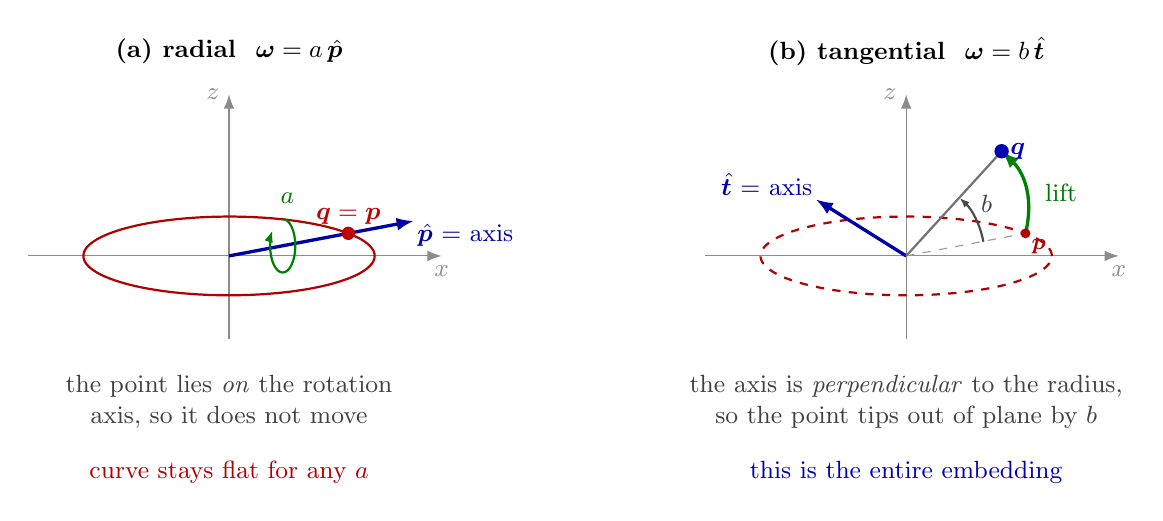
\begin{tikzpicture}[scale=1.0]

%---------------- panel (a): radial component -----------------
\begin{scope}[xshift=-4.3cm]
  \node[font=\bfseries\small] at (0,2.60) {(a) radial \ $\bm\omega = a\,\phat$};
  \draw[-{Latex[length=1.8mm]}, black!45] (-2.55,0) -- (2.70,0) node[below,font=\small] {$x$};
  \draw[-{Latex[length=1.8mm]}, black!45] (0,-1.05) -- (0,2.05) node[left,font=\small] {$z$};
  \draw[thick, red!70!black] plot[domain=0:360,samples=100] ({1.85*cos(\x)},{0.50*sin(\x)});
  \pgfmathsetmacro{\tt}{35}
  \coordinate (O) at (0,0);
  \coordinate (P) at ({1.85*cos(\tt)},{0.50*sin(\tt)});
  % rotation axis: the radius itself, extended
  \draw[blue!65!black, very thick, -{Latex[length=2.2mm]}] (O) -- ($(O)!1.55!(P)$);
  \node[blue!65!black, font=\small, below right, inner sep=1pt] at ($(O)!1.55!(P)$) {$\phat$ = axis};
  % barrel-roll arcs around the axis
  \draw[green!50!black, thick, -{Latex[length=1.5mm]}]
        ($(P)!0.55!(O)$) ++(0,0.34) arc (90:-215:0.16 and 0.34);
  \node[green!45!black, font=\small] at ($(P)!0.55!(O)+(0.06,0.60)$) {$a$};
  \fill[red!75!black] (P) circle (2.4pt);
  \node[red!75!black, font=\small, above, inner sep=3pt] at (P) {$\q=\pv$};
  \node[font=\small, align=center, black!75] at (0,-1.85)
        {the point lies \emph{on} the rotation\\ axis, so it does not move};
  \node[font=\small, red!70!black, align=center] at (0,-2.75)
        {curve stays flat for any $a$};
\end{scope}

%---------------- panel (b): tangential component -----------------
\begin{scope}[xshift=4.3cm]
  \node[font=\bfseries\small] at (0,2.60) {(b) tangential \ $\bm\omega = b\,\that$};
  \draw[-{Latex[length=1.8mm]}, black!45] (-2.55,0) -- (2.70,0) node[below,font=\small] {$x$};
  \draw[-{Latex[length=1.8mm]}, black!45] (0,-1.05) -- (0,2.05) node[left,font=\small] {$z$};
  \draw[thick, red!70!black, dashed] plot[domain=0:360,samples=100] ({1.85*cos(\x)},{0.50*sin(\x)});
  \pgfmathsetmacro{\tt}{35}
  \coordinate (O) at (0,0);
  \coordinate (P) at ({1.85*cos(\tt)},{0.50*sin(\tt)});
  \coordinate (Q) at ({1.85*cos(\tt)*0.80},{0.50*sin(\tt)*0.80+1.10});
  % axis along tangent (into the picture, drawn to upper-left)
  \draw[blue!65!black, very thick, -{Latex[length=2.2mm]}] (O) -- (-1.15,0.72);
  \node[blue!65!black, font=\small, above left, inner sep=1pt] at (-1.15,0.72) {$\that$ = axis};
  % radius before and after
  \draw[black!40, dashed] (O) -- (P);
  \draw[black!55, thick] (O) -- (Q);
  % lift
  \draw[green!50!black, very thick, -{Latex[length=2.2mm]}] (P) to[bend right=30] (Q);
  \node[green!45!black, font=\small] at ($(P)!0.55!(Q)+(0.62,-0.06)$) {lift};
  % elevation angle marker at origin
  \draw[-{Latex[length=1.3mm]}, black!70, thick] (0.98,0.18) arc (10:47:1.00);
  \node[font=\small, black!75] at (1.02,0.66) {$b$};
  \fill[red!70!black] (P) circle (1.8pt);
  \node[red!70!black, font=\footnotesize, below right, inner sep=2pt] at (P) {$\pv$};
  \fill[blue!70!black] (Q) circle (2.6pt);
  \node[blue!70!black, font=\small, right, inner sep=3pt] at (Q) {$\q$};
  \node[font=\small, align=center, black!75] at (0,-1.85)
        {the axis is \emph{perpendicular} to the radius,\\ so the point tips out of plane by $b$};
  \node[font=\small, blue!70!black, align=center] at (0,-2.75)
        {this is the entire embedding};
\end{scope}

\end{tikzpicture}
\caption{Decomposition of the embedding generator in the moving frame of the
virtual agent. \textbf{(a)} A radial generator $a\phat$ rotates the point about
the very axis it lies on, and therefore does nothing
(Proposition~\ref{prop:radialnoop}); the curve remains flat no matter how large
$a$ is. \textbf{(b)} A tangential generator $b\that$ has an axis perpendicular
to the radius, and lifts the point out of the plane by exactly the elevation
angle $b$ (Proposition~\ref{prop:tangential}). All useful embedding is generated
by $b$; $a$ is wasted authority --- and, as \S\ref{sec:azimuth} shows, actively
harmful.}
\label{fig:decomposition}
\end{figure}

\subsection{Worked example: decomposing a candidate generator}
\label{sec:modelB}

The decomposition \eqref{eq:decomp} is not an extra modelling choice. Because
$\omega_z = 0$, the generator already lies in the span of $\{\phat,\that\}$, so
resolving it there is an exact change of basis --- a planar rotation by
$-\theta$:
\begin{equation}
\begin{bmatrix} a(\theta) \\ b(\theta) \end{bmatrix}
=
\begin{bmatrix} \cos\theta & \sin\theta \\ -\sin\theta & \cos\theta \end{bmatrix}
\begin{bmatrix} \omega_x(\theta) \\ \omega_y(\theta) \end{bmatrix}.
\label{eq:abrotation}
\end{equation}
Nothing is added and nothing is lost; what changes is that the two components
can now be read separately. It is worth carrying a concrete case through.

Consider the candidate generator
\begin{equation}
\bm\omega_B(\theta) = \big[\ 0.6\cos2\theta,\ \ 0.6\cos^2\theta,\ \ 0\ \big]^\top ,
\label{eq:modelB}
\end{equation}
arrived at by the usual route of choosing two smooth $2\pi$-periodic functions
for $\omega_x$ and $\omega_y$ and inspecting the resulting curve. Substituting
into \eqref{eq:abrotation} and using $0.6\cos^2\theta = 0.3(1+\cos2\theta)$,
\begin{align}
a_B(\theta) &= \ \ \,0.6\cos2\theta\,\cos\theta + 0.3\,(1+\cos2\theta)\,\sin\theta, \label{eq:aB}\\
b_B(\theta) &= -0.6\cos2\theta\,\sin\theta + 0.3\,(1+\cos2\theta)\,\cos\theta . \label{eq:bB}
\end{align}
Figure~\ref{fig:modelB} plots the two components over one revolution, together
with the azimuth error they produce; Table~\ref{tab:modelB} collects the
figures. Both $a_B$ and $b_B$ change sign under $\theta\mapsto\theta+\pi$, so
by \eqref{eq:psiexact} the azimuth error is $\pi$-periodic even though the
generator is not.

\begin{table}[htbp]
\centering
\caption{Model B \eqref{eq:modelB} resolved in the moving frame. Roughly a
third of the generator does no geometric work, and that third is what corrupts
the phase.}
\label{tab:modelB}
\begin{tabular}{lll}
\toprule
Quantity & Value & Interpretation \\
\midrule
$\max_\theta|a_B|$ & $0.657$ rad $=37.6^\circ$ & radial: contributes no shape (Prop.~\ref{prop:radialnoop}) \\
$\max_\theta|b_B|$ & $0.676$ rad $=38.8^\circ$ & tangential: the actual elevation profile \\
$\int a_B^2 \,/\, \int(a_B^2+b_B^2)$ & $35.7\%$ & fraction of the generator that is wasted \\
elevation range & $\pm 0.612\,r$ & out-of-plane excursion \\
$\max_\theta|\psi|$ & $11.6^\circ$ & \emph{systematic} phase error, not noise \\
RMS $\psi$ & $4.9^\circ$ & \\
\bottomrule
\end{tabular}
\end{table}

\begin{figure}[htbp]
\centering
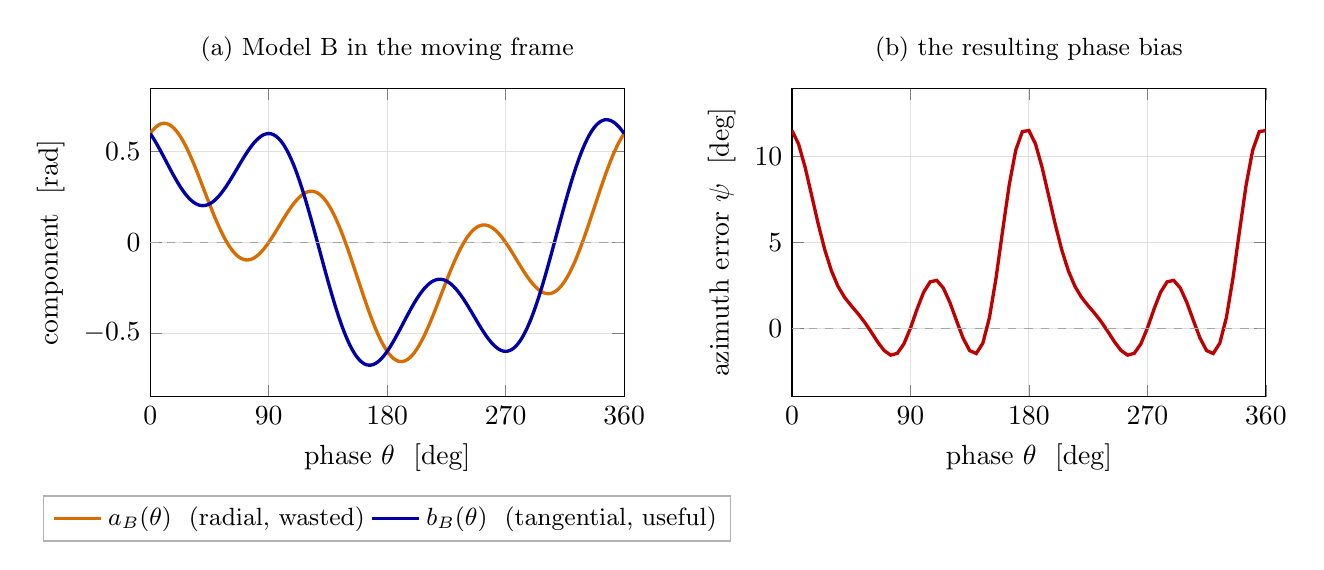
\begin{tikzpicture}

\begin{scope}
\begin{axis}[
  width=7.6cm, height=5.5cm,
  xlabel={phase $\theta$ \ [deg]}, ylabel={component \ [rad]},
  domain=0:360, samples=220,
  xmin=0, xmax=360, ymin=-0.85, ymax=0.85,
  xtick={0,90,180,270,360},
  legend style={at={(0.5,-0.32)}, anchor=north, legend columns=2, draw=black!30, font=\small},
  legend cell align=left,
  grid=both, grid style={black!12},
  every axis plot/.append style={very thick},
  title={\small (a) Model B in the moving frame},
]
\addplot[orange!85!black] {0.6*cos(2*x)*cos(x) + 0.3*(1+cos(2*x))*sin(x)};
\addlegendentry{$a_B(\theta)$ \ (radial, wasted)}
\addplot[blue!65!black] {-0.6*cos(2*x)*sin(x) + 0.3*(1+cos(2*x))*cos(x)};
\addlegendentry{$b_B(\theta)$ \ (tangential, useful)}
\addplot[black!35, dashed, thin] {0};
\end{axis}
\end{scope}

\begin{scope}[xshift=8.15cm]
\begin{axis}[
  width=7.6cm, height=5.5cm,
  xlabel={phase $\theta$ \ [deg]}, ylabel={azimuth error $\psi$ \ [deg]},
  xmin=0, xmax=360, ymin=-4, ymax=14,
  xtick={0,90,180,270,360},
  grid=both, grid style={black!12},
  every axis plot/.append style={very thick},
  title={\small (b) the resulting phase bias},
]
\addplot[red!75!black] coordinates {
(0,11.532) (5,10.746) (10,9.382) (15,7.733) (20,6.058) (25,4.555)
(30,3.339) (35,2.436) (40,1.794) (45,1.309) (50,0.862) (55,0.367)
(60,-0.202) (65,-0.796) (70,-1.303) (75,-1.574) (80,-1.470) (85,-0.925)
(90,-0.000) (95,1.102) (100,2.092) (105,2.703) (110,2.787) (115,2.343)
(120,1.493) (125,0.437) (130,-0.584) (135,-1.309) (140,-1.480) (145,-0.878)
(150,0.612) (155,2.909) (160,5.667) (165,8.341) (170,10.385) (175,11.466)
(180,11.532) (185,10.746) (190,9.382) (195,7.733) (200,6.058) (205,4.555)
(210,3.339) (215,2.436) (220,1.794) (225,1.309) (230,0.862) (235,0.367)
(240,-0.202) (245,-0.796) (250,-1.303) (255,-1.574) (260,-1.470) (265,-0.925)
(270,-0.000) (275,1.102) (280,2.092) (285,2.703) (290,2.787) (295,2.343)
(300,1.493) (305,0.437) (310,-0.584) (315,-1.309) (320,-1.480) (325,-0.878)
(330,0.612) (335,2.909) (340,5.667) (345,8.341) (350,10.385) (355,11.466)
(360,11.532)
};
\addplot[black!35, dashed, thin] coordinates {(0,0) (360,0)};
\end{axis}
\end{scope}

\end{tikzpicture}
\caption{A candidate generator, resolved. \textbf{(a)} Model B
\eqref{eq:modelB} has radial and tangential components of comparable size:
$35.7\%$ of it is radial and therefore does nothing to the shape of the curve
(Proposition~\ref{prop:radialnoop}). \textbf{(b)} That idle component is not
free. By Proposition~\ref{prop:azimuth} it shears the azimuth away from the
phase by up to $11.6^\circ$ --- a smooth, repeatable, phase-dependent bias that
no amount of filtering removes, since it is a property of the trajectory
definition rather than of the sensor. Compare the $\sigma_\theta$ budget of
Table~\ref{tab:sizing}: the modelling error alone is comparable to the entire
measurement error.}
\label{fig:modelB}
\end{figure}

\subsection{Repairing a generator, and designing one directly}
\label{sec:repair}

Given an existing generator, two repairs are available.

\begin{enumerate}
\item \textbf{Drop the radial part.} Keep $b_B(\theta)$ from \eqref{eq:bB} and
set $a\equiv0$. The azimuth error vanishes identically. The elevation deepens
slightly, from $\pm0.612\,r$ to $\pm0.626\,r$, because the radial component was
damping it: by \eqref{eq:components} the vertical coordinate is
$-r\,(b/\phi)\sin\phi$ with $\phi = \sqrt{a^2+b^2}$, which reduces to
$-r\sin b$ only when $a=0$.

\item \textbf{Preserve the elevation profile exactly.} If the original
out-of-plane excursion is to be reproduced, set
\begin{equation}
b_{\text{new}}(\theta) = \arcsin\!\big(-z_B(\theta)/r\big),
\qquad
z_B(\theta) = -r\,\frac{b_B(\theta)}{\phi_B(\theta)}\sin\phi_B(\theta) .
\label{eq:repair}
\end{equation}
For Model B this gives $\max|b_{\text{new}}| = 0.658$ rad $=37.7^\circ$,
comfortably inside Assumption~\ref{as:polar}, reproduces the elevation to
machine precision, and yields azimuth error below $10^{-13}$ degrees. The
resulting curve is Model B's with the azimuth shear removed: the same elevation
profile, re-parameterized so that phase and azimuth coincide.
\end{enumerate}

In new designs neither repair is needed, because the construction can be run in
the useful direction. Rather than choosing $(\omega_x,\omega_y)$ and inspecting
the curve that results, choose the elevation profile $b(\theta)$ and read off
the generator:
\begin{equation}
\boxed{\;
\bm\omega(\theta) = b(\theta)\,\that(\theta)
\quad\Longleftrightarrow\quad
\omega_x(\theta) = -b(\theta)\sin\theta,
\qquad
\omega_y(\theta) = +b(\theta)\cos\theta .
\;}
\label{eq:designforward}
\end{equation}
This is the same class of object --- two components, $\omega_z=0$ --- but
constrained to one free function instead of two, and the function retained is
the one with a direct geometric meaning: $b(\theta)$ is the elevation angle of
the vehicle above the plane of the virtual circle. Peak excursion is
$r\sin b_{\max}$, which feeds straight into the clearance rule of
\S\ref{sec:hzero} without simulation. Simple profiles behave as their harmonic
number suggests: $b_0\cos\theta$ gives one up-lobe and one down-lobe,
$b_0\cos2\theta$ the four-crossing saddle used in the figures of this note, and
$b_0\cos3\theta$ a three-fold symmetric curve that pairs naturally with $n=3$.

A final practical consequence: under \eqref{eq:designforward} the matrix
exponential is never evaluated. The normal form \eqref{eq:normalform} gives
$\q(\theta)$ in three trigonometric calls, agreeing with the $\exp(\skewm{\cdot})$
route to $2.5\times10^{-16}$, and it differentiates in closed form for the
filter Jacobian of \S\ref{sec:ekf}.

\begin{remark}[A note on $\omega_z$]
\label{rem:omegaz}
The constraint that matters is $\bm\omega \perp \pv$, not $\omega_z = 0$; the
latter is automatic in the intended construction and is often justified on the
wrong grounds. A vertical component does not tilt anything:
$\exp\!\big(\skewm{\omega_z\ez}\big)\pv(\theta) = \pv(\theta + \omega_z)$, a
pure azimuth shift with no effect on the shape of the curve and a
one-for-one contribution to the azimuth error. The three components thus have
three distinct roles --- $\omega_z$ reparameterizes the phase, $a$ wastes
authority and shears the phase, and $b$ alone generates the curve.
\end{remark}


\subsection{Designing an elevation profile from waypoints}
\label{sec:waypoints}

Because \eqref{eq:designforward} reduces the whole trajectory design to the
choice of one scalar $2\pi$-periodic function, specifying a trajectory by
waypoints becomes an ordinary periodic scalar interpolation problem. This
subsection sets out the procedure, the family of curves it can reach, and the
quantity that limits how much detail is worth asking for.

\subsubsection*{The reachable family, and projection onto it}

The construction \eqref{eq:designforward} generates precisely the closed curves
that are
\emph{(i)} contained in the sphere $\norm{\q-\cv}=r$,
\emph{(ii)} \emph{graphs over azimuth} --- exactly one point at each $\theta$, and
\emph{(iii)} bounded away from the poles, $|b|<\pi/2$ (Assumption~\ref{as:polar}).
This is a real restriction. A curve that reverses in azimuth, or that varies
its distance from the encirclement centre, is not reachable; what is bought in
exchange is that phase and azimuth coincide exactly
(Corollary~\ref{cor:exact}).

Arbitrary waypoints $\bm w_1,\dots,\bm w_N \in \R^3$ must therefore first be
projected onto that family. Each contributes an (azimuth, elevation) pair,
\begin{equation}
\theta_i = \operatorname{atan2}\big(w_{i,y}-c_y,\ w_{i,x}-c_x\big),
\qquad
b_i = -\arcsin\!\left(\frac{w_{i,z}-c_z}{\norm{\bm w_i - \cv}}\right),
\label{eq:wpproject}
\end{equation}
while the range $\norm{\bm w_i-\cv}$ is discarded. The consequence is worth
stating plainly: \emph{the curve matches each waypoint's direction from the
encirclement centre exactly, and its distance not at all}. The residual is
purely radial, of size $\big|\norm{\bm w_i-\cv}-r\big|$, and is known in advance
from \eqref{eq:wpproject} --- so it can be reported to the user at specification
time rather than discovered in flight. Table~\ref{tab:wp} shows this for the
six-waypoint example used throughout this subsection.

\begin{table}[htbp]
\centering
\caption{Six sketched waypoints projected onto the design family by
\eqref{eq:wpproject}, with $\cv = [0,0,1]^\top$ and $r=1$~m. The azimuth and
elevation are matched exactly; the radial slip is the price, and it is known
before the vehicle flies.}
\label{tab:wp}
\begin{tabular}{lccccc}
\toprule
& $\theta_i$ [deg] & $b_i$ [deg] & $\norm{\bm w_i-\cv}$ [m] & radial slip [m] \\
\midrule
$\bm w_1$ & $\ \ \,5.4$ & $-18.4$ & $1.111$ & $+0.111$ \\
$\bm w_2$ & $\ 78.1$    & $\ -2.9$ & $0.972$ & $-0.028$ \\
$\bm w_3$ & $158.7$     & $+16.2$ & $1.005$ & $+0.005$ \\
$\bm w_4$ & $223.0$     & $\ -5.6$ & $1.031$ & $+0.031$ \\
$\bm w_5$ & $277.8$     & $-22.1$ & $1.198$ & $+0.198$ \\
$\bm w_6$ & $337.6$     & $-16.9$ & $0.961$ & $-0.039$ \\
\bottomrule
\end{tabular}
\end{table}

\subsubsection*{Trigonometric fitting}

Assumption~\ref{as:closed} requires $b$ to be $2\pi$-periodic, so the natural
basis is the truncated Fourier series
\begin{equation}
b(\theta) = \beta_0 + \sum_{k=1}^{K}\big(\alpha_k\cos k\theta + \beta_k\sin k\theta\big),
\label{eq:fourierb}
\end{equation}
with $2K+1$ coefficients $\bm x = [\beta_0,\alpha_1,\beta_1,\dots,\alpha_K,\beta_K]^\top$
obtained from the linear least-squares problem $\min_{\bm x}\norm{M\bm x - \bm b}$,
where
\begin{equation}
M_{i\cdot} = \big[\,1,\ \cos\theta_i,\ \sin\theta_i,\ \dots,\ \cos K\theta_i,\ \sin K\theta_i\,\big],
\qquad
\bm b = [b_1,\dots,b_N]^\top .
\label{eq:fitls}
\end{equation}
With $2K+1 \ge N$ and distinct $\theta_i$ the waypoints are interpolated
exactly; below that they are approximated. Periodicity, and hence closedness of
the curve, is automatic --- it is a property of the basis, not a constraint to
be imposed. If the $\theta_i$ happen to be equispaced, \eqref{eq:fitls} reduces
to a discrete Fourier transform.

\begin{algorithm}[htbp]
\caption{Elevation profile from waypoints}
\label{alg:waypoints}
\begin{algorithmic}[1]
\Require waypoints $\bm w_1,\dots,\bm w_N$; centre $\cv=h\ez$; radius $r$;
         clearance margin $\epsilon$; peak vertical acceleration $a_{\max}$;
         phase rate $\omega$; fit tolerance $\tau$
\Ensure  elevation profile $b(\theta)$, or failure
\State $\theta_i \gets \operatorname{atan2}(w_{i,y}-c_y,\ w_{i,x}-c_x)$,\quad
       $b_i \gets -\arcsin\!\big((w_{i,z}-c_z)/\norm{\bm w_i-\cv}\big)$ \Comment{project, Eq.~\eqref{eq:wpproject}}
\State report radial slips $\big|\norm{\bm w_i-\cv}-r\big|$ to the user
\State sort by $\theta_i$; \textbf{abort} if any two $\theta_i$ coincide \Comment{graph-over-azimuth}
\For{$K = 1,2,3,\dots$}
  \State assemble $M$ by \eqref{eq:fitls} and solve $\min\norm{M\bm x-\bm b}$
  \State evaluate $b,b',b''$ on a dense grid in $[0,2\pi)$
  \State \textbf{reject} if $\max_\theta|b| \ge \pi/2$ \Comment{Assumption~\ref{as:polar}}
  \State \textbf{reject} if $h - r\sin\big(\max_\theta b\big) \le \epsilon$ \Comment{clearance, Eq.~\eqref{eq:clearance}}
  \State \textbf{reject} if $r\omega^2\max_\theta\big|b''\cos b - b'^2\sin b\big| > a_{\max}$ \Comment{actuation, Eq.~\eqref{eq:zaccel}}
  \State \textbf{accept and break} if the waypoint residual $\le \tau$
\EndFor
\State \Return $\bm\omega(\theta) = b(\theta)\that(\theta)$, or equivalently evaluate
       $\q(\theta)$ directly from the normal form \eqref{eq:normalform}
\end{algorithmic}
\end{algorithm}

Three points about Algorithm~\ref{alg:waypoints} deserve emphasis. The
acceptance tests in lines 7--9 are evaluated on a \emph{dense grid}, not at the
waypoints: a trigonometric interpolant overshoots between its data, and it is
the overshoot that grounds the vehicle. In the worked example the fitted
$\max_\theta|b| = 23.2^\circ$ exceeds the largest waypoint elevation of
$22.1^\circ$. Second, $K$ is increased from below and the loop exits at the
first acceptable fit, because --- as shown next --- the cost of harmonic order
is steep and the smallest adequate $K$ is the right one. Third, no step
requires a matrix exponential.

\subsubsection*{What the fits look like}

Figure~\ref{fig:wpfit} shows the fits and the resulting curves. With $N=6$
waypoints, $K=3$ ($2K+1=7$ coefficients) interpolates exactly; $K=2$ leaves
$1.04^\circ$ RMS and $K=1$ leaves $4.15^\circ$, the latter visibly a
single-lobe tilt that ignores the finer structure. The right-hand panel shows
why one does not simply take $K$ large: the waypoint residual saturates at zero
by $K=3$, while the peak vertical acceleration keeps climbing.

\begin{figure}[htbp]
\centering
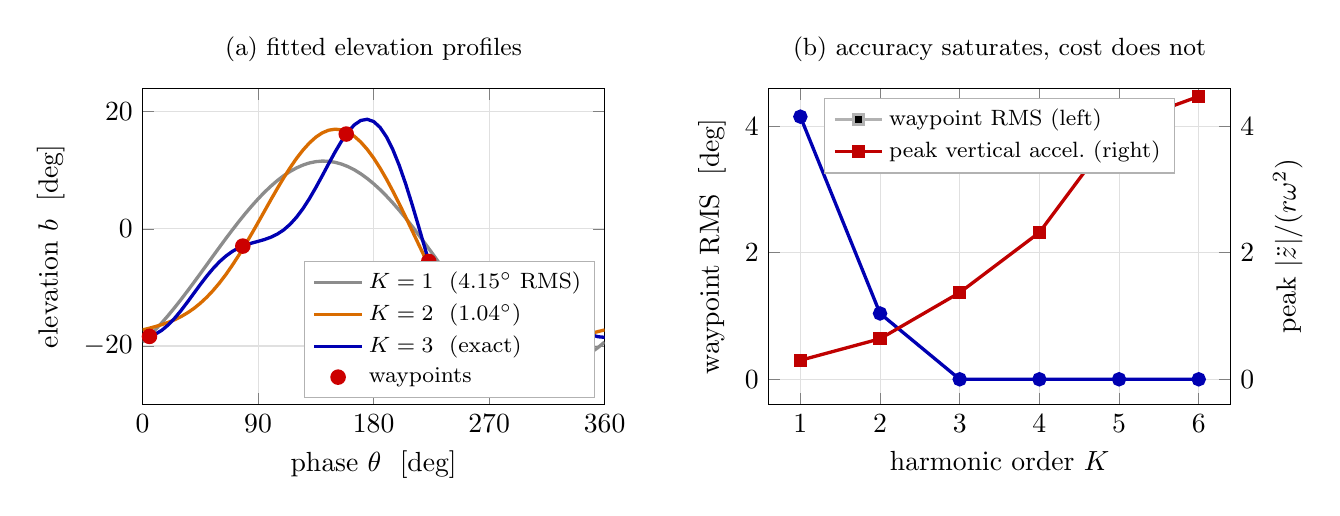
\begin{tikzpicture}

\begin{scope}
\begin{axis}[
  width=7.45cm, height=5.6cm,
  xlabel={phase $\theta$ \ [deg]}, ylabel={elevation $b$ \ [deg]},
  xmin=0, xmax=360, ymin=-30, ymax=24,
  xtick={0,90,180,270,360},
  legend style={at={(0.98,0.02)}, anchor=south east, draw=black!30, font=\footnotesize},
  legend cell align=left, grid=both, grid style={black!12},
  every axis plot/.append style={very thick},
  title={\small (a) fitted elevation profiles},
]
\addplot[black!45] coordinates {
(0,-19.33) (5,-18.33) (10,-17.23) (15,-16.04) (20,-14.78) (25,-13.45)
(30,-12.06) (35,-10.62) (40,-9.15) (45,-7.65) (50,-6.14) (55,-4.62)
(60,-3.12) (65,-1.63) (70,-0.18) (75,1.23) (80,2.59) (85,3.88)
(90,5.10) (95,6.24) (100,7.28) (105,8.23) (110,9.07) (115,9.79)
(120,10.40) (125,10.88) (130,11.24) (135,11.46) (140,11.56) (145,11.52)
(150,11.35) (155,11.05) (160,10.62) (165,10.07) (170,9.39) (175,8.60)
(180,7.70) (185,6.70) (190,5.60) (195,4.42) (200,3.16) (205,1.82)
(210,0.44) (215,-1.00) (220,-2.47) (225,-3.97) (230,-5.49) (235,-7.00)
(240,-8.51) (245,-9.99) (250,-11.45) (255,-12.86) (260,-14.21) (265,-15.51)
(270,-16.73) (275,-17.86) (280,-18.91) (285,-19.85) (290,-20.69) (295,-21.42)
(300,-22.02) (305,-22.51) (310,-22.86) (315,-23.09) (320,-23.18) (325,-23.14)
(330,-22.98) (335,-22.68) (340,-22.25) (345,-21.69) (350,-21.02) (355,-20.23)
(360,-19.33)
}; \addlegendentry{$K=1$ \ ($4.15^\circ$ RMS)}
\addplot[orange!85!black] coordinates {
(0,-17.26) (5,-16.98) (10,-16.68) (15,-16.35) (20,-15.97) (25,-15.52)
(30,-14.98) (35,-14.34) (40,-13.59) (45,-12.70) (50,-11.68) (55,-10.52)
(60,-9.22) (65,-7.78) (70,-6.20) (75,-4.51) (80,-2.72) (85,-0.85)
(90,1.07) (95,3.02) (100,4.97) (105,6.88) (110,8.71) (115,10.44)
(120,12.03) (125,13.44) (130,14.65) (135,15.64) (140,16.37) (145,16.83)
(150,17.00) (155,16.89) (160,16.48) (165,15.79) (170,14.81) (175,13.57)
(180,12.09) (185,10.38) (190,8.49) (195,6.44) (200,4.27) (205,2.01)
(210,-0.30) (215,-2.61) (220,-4.90) (225,-7.12) (230,-9.26) (235,-11.27)
(240,-13.13) (245,-14.82) (250,-16.33) (255,-17.64) (260,-18.75) (265,-19.67)
(270,-20.38) (275,-20.90) (280,-21.25) (285,-21.44) (290,-21.48) (295,-21.40)
(300,-21.22) (305,-20.96) (310,-20.64) (315,-20.28) (320,-19.90) (325,-19.51)
(330,-19.13) (335,-18.77) (340,-18.43) (345,-18.11) (350,-17.81) (355,-17.53)
(360,-17.26)
}; \addlegendentry{$K=2$ \ ($1.04^\circ$)}
\addplot[blue!70!black] coordinates {
(0,-18.52) (5,-18.38) (10,-17.98) (15,-17.32) (20,-16.40) (25,-15.26)
(30,-13.94) (35,-12.50) (40,-11.00) (45,-9.51) (50,-8.08) (55,-6.77)
(60,-5.61) (65,-4.64) (70,-3.85) (75,-3.25) (80,-2.79) (85,-2.44)
(90,-2.14) (95,-1.83) (100,-1.43) (105,-0.90) (110,-0.18) (115,0.78)
(120,1.99) (125,3.45) (130,5.15) (135,7.04) (140,9.05) (145,11.11)
(150,13.11) (155,14.96) (160,16.53) (165,17.74) (170,18.49) (175,18.69)
(180,18.32) (185,17.32) (190,15.71) (195,13.52) (200,10.81) (205,7.66)
(210,4.17) (215,0.47) (220,-3.30) (225,-7.02) (230,-10.56) (235,-13.80)
(240,-16.65) (245,-19.02) (250,-20.87) (255,-22.17) (260,-22.94) (265,-23.21)
(270,-23.03) (275,-22.49) (280,-21.67) (285,-20.67) (290,-19.60) (295,-18.54)
(300,-17.59) (305,-16.80) (310,-16.22) (315,-15.89) (320,-15.79) (325,-15.92)
(330,-16.23) (335,-16.68) (340,-17.19) (345,-17.70) (350,-18.13) (355,-18.42)
(360,-18.52)
}; \addlegendentry{$K=3$ \ (exact)}
\addplot[only marks, mark=*, mark size=2.2pt, red!80!black] coordinates {
(5.4,-18.36) (78.1,-2.95) (158.7,16.17) (223.0,-5.57) (277.8,-22.06) (337.6,-16.94)
}; \addlegendentry{waypoints}
\end{axis}
\end{scope}

\begin{scope}[xshift=7.95cm]
\begin{axis}[
  width=7.45cm, height=5.6cm,
  xlabel={harmonic order $K$}, ylabel={waypoint RMS \ [deg]},
  xmin=0.6, xmax=6.4, ymin=-0.4, ymax=4.6,
  xtick={1,2,3,4,5,6},
  axis y line*=left, grid=both, grid style={black!12},
  every axis plot/.append style={very thick, mark=*, mark size=2pt},
  title={\small (b) accuracy saturates, cost does not},
]
\addplot[blue!70!black] coordinates {
(1,4.15) (2,1.04) (3,0.00) (4,0.00) (5,0.00) (6,0.00)
}; \label{plt:resid}
\end{axis}
\begin{axis}[
  width=7.45cm, height=5.6cm,
  xmin=0.6, xmax=6.4, ymin=-0.4, ymax=4.6,
  axis y line*=right, axis x line=none,
  ylabel={peak $|\ddot z|/(r\omega^2)$},
  every axis plot/.append style={very thick, mark=square*, mark size=1.8pt},
  legend style={at={(0.5,0.97)}, anchor=north, draw=black!30, font=\footnotesize},
  legend cell align=left,
]
\addlegendimage{/pgfplots/refstyle=plt:resid}\addlegendentry{waypoint RMS (left)}
\addplot[red!75!black] coordinates {
(1,0.30) (2,0.64) (3,1.37) (4,2.32) (5,4.01) (6,4.47)
}; \addlegendentry{peak vertical accel.\ (right)}
\end{axis}
\end{scope}

\end{tikzpicture}
\caption{Fitting an elevation profile to six waypoints. \textbf{(a)} Truncated
Fourier fits \eqref{eq:fourierb} of increasing order. $K=3$ interpolates the six
waypoints exactly; lower orders approximate. Note that the $K=3$ interpolant
overshoots the extreme waypoint, which is why the clearance test in
Algorithm~\ref{alg:waypoints} is evaluated on a dense grid.
\textbf{(b)} The waypoint residual reaches zero at $K=3$ and cannot improve
further, while the peak vertical acceleration continues to grow roughly as
$K^2$. The smallest adequate $K$ is the correct choice.}
\label{fig:wpfit}
\end{figure}

\begin{figure}[htbp]
\centering
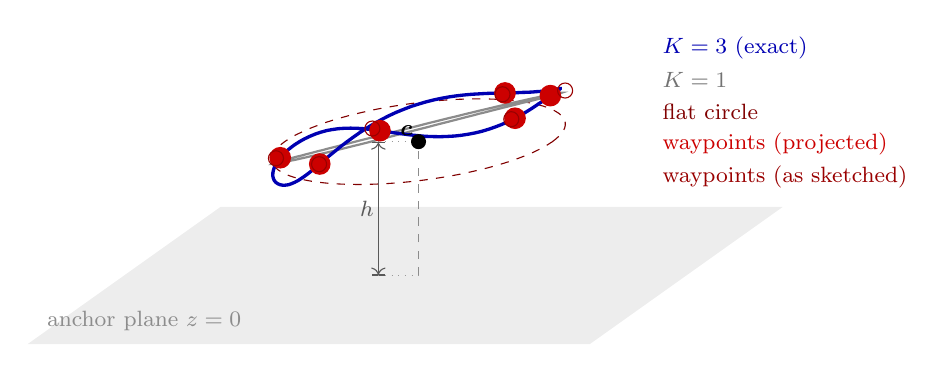
\begin{tikzpicture}[scale=1.7]
  % oblique projection (X,Y,Z) -> (X + 0.45 Y, 0.32 Y + Z), centre c = (0,0,1)
  % z=0 plane, X in [-2.2,2.0], Y in [-1.6,1.6] under the same projection
  \fill[black!7] (-2.92,-0.512) -- (1.28,-0.512) -- (2.72,0.512) -- (-1.48,0.512) -- cycle;
  \node[black!45, font=\footnotesize] at (-2.05,-0.34) {anchor plane $z=0$};

  % flat reference circle b = 0
  \draw[red!50!black, dashed, thin] plot coordinates {
(1.000,1.000) (1.027,1.021) (1.050,1.042) (1.069,1.062) (1.082,1.083)
(1.092,1.103) (1.096,1.122) (1.096,1.142) (1.091,1.160) (1.081,1.178)
(1.067,1.195) (1.049,1.211) (1.025,1.226) (0.998,1.241) (0.966,1.254)
(0.930,1.266) (0.890,1.277) (0.846,1.287) (0.798,1.296) (0.748,1.303)
(0.693,1.309) (0.636,1.314) (0.577,1.317) (0.514,1.319) (0.450,1.320)
(0.384,1.319) (0.316,1.317) (0.246,1.314) (0.176,1.309) (0.105,1.303)
(0.033,1.296) (-0.039,1.287) (-0.110,1.277) (-0.181,1.266) (-0.252,1.254)
(-0.321,1.241) (-0.389,1.226) (-0.455,1.211) (-0.519,1.195) (-0.581,1.178)
(-0.641,1.160) (-0.698,1.142) (-0.752,1.122) (-0.802,1.103) (-0.849,1.083)
(-0.893,1.062) (-0.933,1.042) (-0.968,1.021) (-1.000,1.000) (-1.027,0.979)
(-1.050,0.958) (-1.069,0.938) (-1.082,0.917) (-1.092,0.897) (-1.096,0.878)
(-1.096,0.858) (-1.091,0.840) (-1.081,0.822) (-1.067,0.805) (-1.049,0.789)
(-1.025,0.774) (-0.998,0.759) (-0.966,0.746) (-0.930,0.734) (-0.890,0.723)
(-0.846,0.713) (-0.798,0.704) (-0.748,0.697) (-0.693,0.691) (-0.636,0.686)
(-0.577,0.683) (-0.514,0.681) (-0.450,0.680) (-0.384,0.681) (-0.316,0.683)
(-0.246,0.686) (-0.176,0.691) (-0.105,0.697) (-0.033,0.704) (0.039,0.713)
(0.110,0.723) (0.181,0.734) (0.252,0.746) (0.321,0.759) (0.389,0.774)
(0.455,0.789) (0.519,0.805) (0.581,0.822) (0.641,0.840) (0.698,0.858)
(0.752,0.878) (0.802,0.897) (0.849,0.917) (0.893,0.938) (0.933,0.958)
(0.968,0.979) (1.000,1.000)
};
  % K = 1 fit
  \draw[black!45, thick] plot coordinates {
(0.944,1.331) (0.968,1.337) (0.990,1.343) (1.009,1.348) (1.026,1.352)
(1.040,1.356) (1.052,1.359) (1.060,1.362) (1.065,1.364) (1.068,1.365)
(1.067,1.365) (1.063,1.365) (1.056,1.364) (1.046,1.363) (1.033,1.360)
(1.016,1.357) (0.997,1.354) (0.974,1.349) (0.948,1.344) (0.920,1.338)
(0.888,1.331) (0.854,1.324) (0.818,1.316) (0.778,1.307) (0.737,1.298)
(0.693,1.288) (0.648,1.277) (0.600,1.266) (0.551,1.254) (0.500,1.242)
(0.448,1.230) (0.395,1.217) (0.341,1.204) (0.286,1.190) (0.230,1.177)
(0.174,1.163) (0.118,1.149) (0.061,1.135) (0.004,1.120) (-0.052,1.106)
(-0.108,1.092) (-0.164,1.078) (-0.220,1.064) (-0.274,1.050) (-0.328,1.036)
(-0.381,1.023) (-0.433,1.010) (-0.484,0.997) (-0.534,0.984) (-0.582,0.972)
(-0.628,0.960) (-0.674,0.949) (-0.717,0.937) (-0.759,0.927) (-0.799,0.916)
(-0.836,0.907) (-0.872,0.897) (-0.905,0.889) (-0.936,0.881) (-0.965,0.873)
(-0.991,0.866) (-1.014,0.860) (-1.035,0.854) (-1.053,0.849) (-1.067,0.844)
(-1.079,0.840) (-1.088,0.837) (-1.093,0.835) (-1.096,0.833) (-1.095,0.833)
(-1.091,0.832) (-1.084,0.833) (-1.073,0.835) (-1.060,0.837) (-1.043,0.840)
(-1.023,0.844) (-1.000,0.848) (-0.974,0.853) (-0.945,0.860) (-0.914,0.866)
(-0.880,0.874) (-0.843,0.882) (-0.805,0.891) (-0.764,0.900) (-0.721,0.911)
(-0.676,0.921) (-0.630,0.932) (-0.582,0.944) (-0.533,0.956) (-0.482,0.969)
(-0.431,0.981) (-0.379,0.994) (-0.326,1.008) (-0.273,1.021) (-0.219,1.035)
(-0.165,1.049) (-0.112,1.063) (-0.058,1.077) (-0.004,1.091) (0.049,1.104)
(0.102,1.118) (0.155,1.132) (0.207,1.145) (0.258,1.158) (0.308,1.171)
(0.358,1.184) (0.406,1.196) (0.454,1.209) (0.501,1.220) (0.546,1.232)
(0.590,1.243) (0.633,1.254) (0.674,1.264) (0.714,1.274) (0.753,1.284)
(0.789,1.293) (0.824,1.301) (0.857,1.309) (0.888,1.317) (0.917,1.324)
(0.944,1.331)
};
  % K = 3 fit
  \draw[blue!70!black, very thick] plot coordinates {
(0.948,1.318) (0.970,1.333) (0.989,1.346) (1.006,1.358) (1.021,1.368)
(1.033,1.377) (1.044,1.384) (1.051,1.389) (1.057,1.393) (1.059,1.395)
(1.059,1.396) (1.056,1.396) (1.049,1.395) (1.040,1.394) (1.027,1.391)
(1.011,1.388) (0.992,1.385) (0.970,1.382) (0.945,1.379) (0.917,1.376)
(0.885,1.374) (0.852,1.371) (0.815,1.369) (0.777,1.368) (0.736,1.366)
(0.692,1.365) (0.647,1.364) (0.600,1.363) (0.552,1.362) (0.501,1.360)
(0.450,1.357) (0.397,1.354) (0.343,1.349) (0.288,1.343) (0.232,1.335)
(0.176,1.325) (0.119,1.313) (0.062,1.299) (0.004,1.282) (-0.053,1.264)
(-0.110,1.242) (-0.167,1.219) (-0.223,1.193) (-0.279,1.164) (-0.333,1.134)
(-0.386,1.102) (-0.437,1.069) (-0.487,1.034) (-0.535,0.999) (-0.581,0.964)
(-0.624,0.929) (-0.666,0.895) (-0.705,0.862) (-0.741,0.830) (-0.776,0.801)
(-0.809,0.774) (-0.840,0.750) (-0.870,0.729) (-0.897,0.711) (-0.924,0.697)
(-0.949,0.686) (-0.973,0.678) (-0.996,0.675) (-1.017,0.675) (-1.036,0.679)
(-1.052,0.686) (-1.066,0.696) (-1.078,0.710) (-1.085,0.727) (-1.089,0.746)
(-1.088,0.768) (-1.083,0.791) (-1.074,0.817) (-1.059,0.843) (-1.041,0.870)
(-1.018,0.898) (-0.991,0.925) (-0.960,0.951) (-0.927,0.976) (-0.891,0.999)
(-0.852,1.021) (-0.812,1.040) (-0.771,1.057) (-0.729,1.071) (-0.686,1.083)
(-0.642,1.091) (-0.598,1.097) (-0.553,1.100) (-0.507,1.101) (-0.461,1.100)
(-0.414,1.097) (-0.366,1.092) (-0.317,1.086) (-0.267,1.079) (-0.216,1.071)
(-0.165,1.064) (-0.112,1.057) (-0.058,1.050) (-0.004,1.045) (0.050,1.040)
(0.105,1.038) (0.160,1.037) (0.214,1.039) (0.268,1.042) (0.322,1.048)
(0.374,1.056) (0.425,1.066) (0.475,1.078) (0.524,1.093) (0.571,1.109)
(0.615,1.126) (0.658,1.144) (0.699,1.164) (0.738,1.184) (0.775,1.205)
(0.809,1.225) (0.841,1.245) (0.871,1.265) (0.899,1.284) (0.925,1.301)
(0.948,1.318)
};

  % centre and altitude
  \draw[dashed, black!45] (0,0) -- (0,1.06);
  \draw[|<->|, black!65] (-0.30,0) -- node[left,font=\footnotesize,inner sep=1.5pt] {$h$} (-0.30,1);
  \draw[dotted, black!40] (-0.30,0) -- (0,0);
  \draw[dotted, black!40] (-0.30,1) -- (0,1);
  \fill[black] (0,1) circle (1.6pt);
  \node[font=\footnotesize, above left, inner sep=2pt] at (0,1) {$\cv$};

  % projected waypoints (on the curve) and raw waypoints
  \foreach \p in {(0.985,1.344), (0.646,1.364), (-0.738,0.833), (-1.033,0.880), (-0.288,1.082), (0.721,1.175)} { \fill[red!80!black] \p circle (2.3pt); }
  \foreach \p in {(1.095,1.382), (0.627,1.354), (-0.743,0.832), (-1.065,0.876), (-0.345,1.098), (0.693,1.168)}  { \draw[red!60!black, thin] \p circle (1.6pt); }

  \node[blue!70!black, font=\footnotesize, right] at (1.75,1.70) {$K=3$ (exact)};
  \node[black!55, font=\footnotesize, right] at (1.75,1.46) {$K=1$};
  \node[red!50!black, font=\footnotesize, right] at (1.75,1.22) {flat circle};
  \node[red!80!black, font=\footnotesize, right] at (1.75,0.98) {waypoints (projected)};
  \node[red!60!black, font=\footnotesize, right] at (1.75,0.74) {waypoints (as sketched)};
\end{tikzpicture}
\caption{The same fits as closed 3D curves, in oblique projection, with
$r=1$~m and $h=1$~m. Filled markers are the waypoints after projection
\eqref{eq:wpproject}, which the $K=3$ curve passes through exactly; open
markers are the waypoints as originally sketched. The gap between a filled and
an open marker is purely radial and is the quantity tabulated in
Table~\ref{tab:wp}. The flat circle $b\equiv0$ is shown for reference.}
\label{fig:wp3d}
\end{figure}

\subsubsection*{The tangent norm, and what limits the harmonic order}

One identity governs both the observability and the actuation cost of a chosen
profile.

\begin{proposition}[Tangent norm of the normal form]
\label{prop:tangentnorm}
Under the design rule \eqref{eq:designforward},
\begin{equation}
\norm{\q'(\theta)}^2 = r^2\big(b'(\theta)^2 + \cos^2 b(\theta)\big).
\label{eq:tangentnorm}
\end{equation}
\end{proposition}
\begin{proof}
Differentiate \eqref{eq:normalform}. The $\phat$- and $\that$-components of
$\q'$ are $-r(b'\sin b\cos\theta + \cos b\sin\theta)$ and
$-r(b'\sin b\sin\theta - \cos b\cos\theta)$ respectively, whose squares sum to
$r^2(b'^2\sin^2 b + \cos^2 b)$ after the cross terms cancel; the $\ez$-component
is $-rb'\cos b$, contributing $r^2b'^2\cos^2 b$. Adding gives
$r^2(b'^2\sin^2b + b'^2\cos^2 b + \cos^2 b)$, which is \eqref{eq:tangentnorm}.
\end{proof}

\begin{corollary}[Regularity is automatic]
\label{cor:regularity}
Under \eqref{eq:designforward} with $|b|<\pi/2$, $\norm{\q'} \ge r\cos b > 0$
for every $\theta$. Assumption~\ref{as:regular} therefore needs no separate
verification: it is implied by Assumption~\ref{as:polar}.
\end{corollary}

\begin{corollary}[Detail improves observability]
\label{cor:detailhelps}
By the Fisher bound \eqref{eq:fisherbound}, phase information scales with
$\norm{\q'}^2$, which by \eqref{eq:tangentnorm} is \emph{increasing} in
$|b'|$. A more intricate curve is therefore better localised than a flat one,
not worse.
\end{corollary}

Corollary~\ref{cor:detailhelps} is worth pausing on, because the intuition runs
the other way. In the worked example the $K=3$ fit attains
$\max_\theta\norm{\q'}/r = 1.25$ against $1.04$ for $K=1$, a $44\%$ increase in
Fisher information and roughly a $17\%$ reduction in $\sigma_\theta$. The
elaborate trajectory is the easier one to estimate on.

The binding constraint is instead actuation. With the phase advancing at rate
$\omega$, the vertical coordinate $z = h - r\sin b(\theta)$ has
\begin{equation}
\ddot z = -r\omega^2\Big(b''\cos b - b'^2\sin b\Big),
\label{eq:zaccel}
\end{equation}
and for a single harmonic $b = b_0\cos K\theta$ the derivatives scale as
$|b'|\propto K$ and $|b''|\propto K^2$. Numerically, the peak of
\eqref{eq:zaccel} for $b_0 = 0.3$ grows as $0.29K^2$ to within a percent across
$K=1,\dots,6$. This quadratic growth, not the fit quality, is what sets the
usable harmonic order:
\begin{equation}
\boxed{\ K_{\max} \;\approx\; \sqrt{\frac{a_{\max}}{r\,b_0\,\omega^2}}\ }
\label{eq:Kmax}
\end{equation}
for a peak vertical acceleration budget $a_{\max}$.

\begin{remark}[Shape and control are decoupled]
\label{rem:decoupled}
Because $\theta$ is the azimuth exactly, the profile $b(\theta)$ appears
\emph{nowhere} in the estimator state \eqref{eq:cdstate}, its process model, the
separation definitions \eqref{eq:cdsep}, or the control law. It enters only as
a feedforward evaluation of $\q(\theta)$ and $\q'(\theta)$. The trajectory
shape can therefore be redesigned --- new waypoints, a different $K$ --- without
retuning the filter or the controller. This separation is precisely what a
radial component destroys: with $a\ne0$ the shape leaks into the phase through
$\psi$ (\S\ref{sec:azimuth}) and the decoupling is lost.
\end{remark}

\begin{remark}[Recovering the radial dimension, and what it costs]
\label{rem:varradius}
If the radial slip of Table~\ref{tab:wp} is unacceptable, the construction
generalises to $\q(\theta) = \cv + \rho(\theta)\Rot_e(\theta)\pv(\theta)$ with a
second periodic function $\rho>0$, fitted to $\norm{\bm w_i-\cv}$ by the same
least-squares machinery. Since positive scaling does not change azimuth,
Corollary~\ref{cor:exact} survives intact and all three waypoint degrees of
freedom are matched. What is lost is the sphere: Proposition~\ref{prop:sphere}
fails, and with it the linear on-curve system \eqref{eq:linear} and the free
consistency check \eqref{eq:spherecheck}. The EKF of \S\ref{sec:ekf} and the
initialiser of \S\ref{sec:init} both survive, since neither uses
$\norm{\uv}=r$. The trade is therefore three-degree-of-freedom waypoint
matching against the loss of a fault-detection channel, and the sphere is worth
keeping unless the radial miss is operationally significant.
\end{remark}


\subsection{Regularity assumptions}

Three conditions are used implicitly throughout and are stated once here.

\begin{assumption}[Closedness]
\label{as:closed}
$a(\theta)$ and $b(\theta)$ are $2\pi$-periodic and $C^1$, so that
$\q(\theta+2\pi)=\q(\theta)$ and the curve is closed.
\end{assumption}

\begin{assumption}[Regularity]
\label{as:regular}
$\norm{d\q/d\theta} > 0$ for all $\theta$: the curve has no stall points. A
stall point is unobservable regardless of anchor geometry, since
$\partial d_m/\partial\theta \propto d\q/d\theta$ vanishes there for
\emph{every} $m$ simultaneously.
\end{assumption}

\begin{assumption}[Non-polar embedding]
\label{as:polar}
$|b(\theta)| < \pi/2$ for all $\theta$. This keeps $\cos b > 0$, so the curve
never crosses the poles of the sphere and the map $\theta\mapsto\q$ is injective.
At $|b|=\pi/2$ the point reaches the pole, the azimuth becomes undefined, and
the curve self-intersects.
\end{assumption}

%==================================================================
\section{Phase from Cartesian Position: When Does \texorpdfstring{$\operatorname{atan2}$}{atan2} Work?}
\label{sec:azimuth}
%==================================================================

Suppose trilateration has returned the Cartesian position $\q$. The phase
$\theta$ is defined on the \emph{virtual} circle, so the natural worry is that
the azimuth of the real agent, $\operatorname{atan2}(q_y-c_y,\,q_x-c_x)$, is not
the phase --- the embedding has moved the point, and the amount it moved depends
on the very $\theta$ we are trying to find. This section settles the question
exactly. The answer is more useful than either ``it works'' or ``it doesn't''.

\subsection{The azimuth error in closed form}

\begin{proposition}[Exact azimuth error]
\label{prop:azimuth}
Let $\bm\omega = a\phat + b\that$ with $\phi=\sqrt{a^2+b^2}$, and define the
azimuth error
\begin{equation}
\psi \;\triangleq\; \operatorname{atan2}(q_y - c_y,\ q_x - c_x) \;-\; \theta .
\end{equation}
Then
\begin{equation}
\boxed{\;
\psi(a,b) \;=\; \operatorname{atan2}\!\Big(\,
a\,b\,(1-\cos\phi)\ ,\ \
\phi^2\cos\phi + a^2(1-\cos\phi)\,\Big),
\;}
\label{eq:psiexact}
\end{equation}
which depends on $\theta$ only through $a(\theta)$ and $b(\theta)$. For small
$\phi$,
\begin{equation}
\psi = \tfrac{1}{2}ab + \mathcal{O}(\phi^4).
\label{eq:psismall}
\end{equation}
\end{proposition}
\begin{proof}
Apply Rodrigues \eqref{eq:rodrigues} with $\bm\omega=a\phat+b\that$. Using
$\hat{\bm\omega}^\top\pv = ar/\phi$ and
$\hat{\bm\omega}\times\pv = -(br/\phi)\,\ez$ and resolving in
$\{\phat,\that,\ez\}$:
\begin{align}
(\q-\cv)^\top\phat &= r\Big[\cos\phi + \tfrac{a^2}{\phi^2}(1-\cos\phi)\Big], \\
(\q-\cv)^\top\that &= r\,\tfrac{ab}{\phi^2}(1-\cos\phi), \\
(\q-\cv)^\top\ez   &= -r\,\tfrac{b}{\phi}\sin\phi .
\label{eq:components}
\end{align}
Since $\that$ is $\phat$ rotated by $+\pi/2$ in the $xy$-plane, the azimuth of
$\q-\cv$ exceeds $\theta$ by $\operatorname{atan2}$ of the $\that$-component
over the $\phat$-component. Clearing the common factor $r/\phi^2$ gives
\eqref{eq:psiexact}. Expanding $\cos\phi = 1-\phi^2/2+\mathcal{O}(\phi^4)$ gives
numerator $\to ab\phi^2/2$ and denominator $\to \phi^2$, hence
\eqref{eq:psismall}.
\end{proof}

\begin{corollary}[Exactness of $\operatorname{atan2}$ under a tangential embedding]
\label{cor:exact}
If $a(\theta)\equiv 0$ then $\psi \equiv 0$, and
\begin{equation}
\theta = \operatorname{atan2}(q_y - c_y,\ q_x - c_x)
\end{equation}
\emph{exactly}, for any elevation profile $b(\theta)$ satisfying
Assumption~\ref{as:polar} --- however severe.
\end{corollary}
\begin{proof}
Immediate from \eqref{eq:psiexact}, or directly from the normal form
\eqref{eq:normalform}: the $x$ and $y$ components share the strictly positive
common factor $r\cos b$, which $\operatorname{atan2}$ divides out.
\end{proof}

Corollary~\ref{cor:exact} is the practically important statement, and it is
counter-intuitive enough to be worth restating in words. \emph{The embedding
cannot move a point in azimuth. It moves it in elevation only.} A rotation whose
axis is tangential to the circle tips the point up or down about that tangent;
the shadow of the point on the $xy$-plane slides in and out along the ray
$\phat(\theta)$, but never off it. It follows that the severity of the
embedding is irrelevant to phase recovery, and the implicit fixed-point
inversion $\theta = g(\theta)$ that a general $\Rot_e(\theta)$ appears to demand
is unnecessary.

\begin{remark}[What actually causes azimuth error]
\label{rem:cause}
By \eqref{eq:psiexact}, $\psi \ne 0$ requires \emph{both} $a\ne0$ and $b\ne0$;
to leading order it is the \emph{product} $\tfrac12 ab$. So the culprit is not
the depth of the distortion but the presence of a radial component in the
generator --- a component which, by Proposition~\ref{prop:radialnoop},
contributes nothing to the shape of the curve in the first place. It is pure
cost. Table~\ref{tab:psi} gives the magnitudes; the formula
\eqref{eq:psiexact} was verified against direct numerical evaluation of
\eqref{eq:embedding} and agrees to four decimal places over the whole grid.
\end{remark}

\begin{table}[htbp]
\centering
\caption{Azimuth error $\psi$ in degrees from \eqref{eq:psiexact}. The
$a=0$ row is identically zero for every embedding depth; the error is driven by
the radial component, not by the severity of the distortion.}
\label{tab:psi}
\begin{tabular}{lccc}
\toprule
& $b=0.3$ & $b=0.6$ & $b=1.0$ \\
\midrule
$a = 0$   & $0.00^\circ$ & $0.00^\circ$ & $0.00^\circ$ \\
$a = 0.1$ & $0.89^\circ$ & $2.02^\circ$ & $4.86^\circ$ \\
$a = 0.2$ & $1.78^\circ$ & $4.02^\circ$ & $9.60^\circ$ \\
$a = 0.3$ & $2.66^\circ$ & $5.99^\circ$ & $14.13^\circ$ \\
$a = 0.5$ & $4.36^\circ$ & $9.76^\circ$ & $22.25^\circ$ \\
\bottomrule
\end{tabular}
\end{table}

\subsection{Visualising the azimuth error}

Figure~\ref{fig:azimuth} makes the mechanism and its magnitude visible in one
place. The left panel is a top view: the true phase is the direction of the ray
$\phat(\theta)$, and the question is whether the \emph{shadow} of the real agent
--- its projection onto the $xy$-plane --- lands on that ray. Under a purely
tangential generator it does, always; the shadow slides along the ray by the
factor $\cos b$ but does not rotate off it. A radial component shears the
shadow off the ray by the angle $\psi$. The right panel plots $\psi$ from
\eqref{eq:psiexact} against embedding depth $b$ for several values of the radial
contamination $a$: the $a=0$ trace lies exactly on the axis, and every other
trace grows.

\begin{figure}[htbp]
\centering
\resizebox{\textwidth}{!}{%
\begin{tikzpicture}

%---------------- left panel: the shadow picture ----------------
\begin{scope}[xshift=0cm]
  \node[font=\bfseries\small] at (0.2,3.75) {(a) the shadow on the $xy$-plane};

  % base circle
  \draw[red!55!black, thick, dashed] (0,0) circle (2.5);
  \draw[-{Latex[length=1.8mm]}, black!45] (-3.0,0) -- (3.15,0) node[below,font=\small] {$x$};
  \draw[-{Latex[length=1.8mm]}, black!45] (0,-3.0) -- (0,3.15) node[left,font=\small] {$y$};
  \fill[black] (0,0) circle (1.8pt);
  \node[font=\small, below left, inner sep=2pt] at (0,0) {$\cv$};

  \pgfmathsetmacro{\tt}{36}
  \pgfmathsetmacro{\sh}{1.72}
  \pgfmathsetmacro{\tp}{\tt+32}

  % contaminated ray (drawn first, underneath)
  \draw[orange!85!black, thick, dash pattern=on 3pt off 2pt]
       (0,0) -- ({2.90*cos(\tp)},{2.90*sin(\tp)});

  % true ray
  \draw[very thick, red!70!black, -{Latex[length=2.2mm]}]
       (0,0) -- ({3.05*cos(\tt)},{3.05*sin(\tt)});
  \node[red!70!black, font=\small, right, inner sep=2pt]
       at ({3.05*cos(\tt)},{3.05*sin(\tt)}) {$\phat(\theta)$};

  % virtual agent on the circle
  \fill[red!70!black] ({2.5*cos(\tt)},{2.5*sin(\tt)}) circle (2.4pt);
  \node[red!70!black,font=\footnotesize, below right, inner sep=3pt]
       at ({2.5*cos(\tt)},{2.5*sin(\tt)}) {$\pv(\theta)$};

  % shadow with a = 0 : on the ray, shorter by cos b
  \draw[blue!55!black, thick, dotted]
      ({\sh*cos(\tt)},{\sh*sin(\tt)}) -- ({2.42*cos(\tt)},{2.42*sin(\tt)});
  \fill[blue!70!black] ({\sh*cos(\tt)},{\sh*sin(\tt)}) circle (2.9pt);
  \draw[blue!55!black, thin] ({\sh*cos(\tt)},{\sh*sin(\tt)}) -- (2.55,-1.10);
  \node[blue!70!black, font=\footnotesize, align=left, right, inner sep=2pt]
      at (2.55,-1.10) {shadow,\\ $a=0$};

  % shadow with a != 0 : rotated off the ray
  \fill[orange!85!black] ({\sh*cos(\tp)},{\sh*sin(\tp)}) circle (2.9pt);
  \draw[orange!85!black, thin] ({\sh*cos(\tp)},{\sh*sin(\tp)}) -- (-1.35,2.55);
  \node[orange!85!black, font=\footnotesize, align=right, left, inner sep=2pt]
      at (-1.35,2.55) {shadow,\\ $a\neq0$};

  % psi arc between the two shadows
  \draw[-{Latex[length=1.5mm]}, orange!85!black, very thick]
       ({1.08*cos(\tt)},{1.08*sin(\tt)}) arc ({\tt}:{\tp}:1.08);
  \node[orange!85!black, font=\small] at ({1.42*cos(\tt+16)},{1.42*sin(\tt+16)}) {$\psi$};

  % theta arc
  \draw[-{Latex[length=1.4mm]}, black!70] (0.55,0) arc (0:{\tt}:0.55);
  \node[font=\small] at (0.80,0.20) {$\theta$};

  \node[font=\small, align=center, black!75] at (0.2,-3.60)
     {a tangential embedding shortens the shadow\\ but never rotates it off the ray};
\end{scope}

%---------------- right panel: the quantitative plot ----------------
\begin{scope}[xshift=8.7cm, yshift=-0.55cm]
\begin{axis}[
  width=8.4cm, height=7.0cm,
  xlabel={embedding depth $b$ \ [rad]},
  ylabel={azimuth error $\psi$ \ [deg]},
  xmin=0, xmax=1.2, ymin=-1.2, ymax=26,
  domain=0:1.2, samples=120,
  legend style={at={(0.02,0.98)}, anchor=north west, draw=black!30, font=\small},
  legend cell align=left,
  grid=both, grid style={black!12},
  every axis plot/.append style={very thick},
  title={\small (b) $\psi$ from Eq.~\eqref{eq:psiexact}},
]
\addplot[green!50!black] {psierr(0.0,x)};  \addlegendentry{$a = 0$ \ (exact)}
\addplot[blue!65!black]  {psierr(0.1,x)};  \addlegendentry{$a = 0.1$}
\addplot[purple!70!black]{psierr(0.2,x)};  \addlegendentry{$a = 0.2$}
\addplot[orange!85!black]{psierr(0.3,x)};  \addlegendentry{$a = 0.3$}
\addplot[red!75!black]   {psierr(0.5,x)};  \addlegendentry{$a = 0.5$}
\end{axis}
\end{scope}

\end{tikzpicture}}
\caption{Why the phase is (and is not) the azimuth. \textbf{(a)} Top view. The
embedding tips the agent out of plane about the tangent $\that$, so its shadow
on the $xy$-plane slides \emph{along} the ray $\phat(\theta)$, scaled by
$\cos b$, and the azimuth is unchanged. Only a radial component $a$ shears the
shadow off the ray, by the angle $\psi$. \textbf{(b)} The exact error
\eqref{eq:psiexact}. The $a=0$ curve is identically zero for every embedding
depth: the depth of the distortion is \emph{not} what causes phase error. With
$a\ne 0$ the error grows roughly as $\tfrac12 ab$ and reaches tens of degrees
for aggressive embeddings.}
\label{fig:azimuth}
\end{figure}

\subsection{Design rule, and the fallback if it is violated}

\begin{center}
\fbox{\parbox{0.93\textwidth}{
\textbf{Design rule (embedding).}\; Generate the curve with a purely tangential
generator, $\bm\omega(\theta) = b(\theta)\,\that(\theta)$ with $|b|<\pi/2$.
The radial component contributes no shape (Proposition~\ref{prop:radialnoop}),
damps the elevation actually achieved, and is the sole source of azimuth error
(Proposition~\ref{prop:azimuth}). Under this rule the phase is recovered in
closed form as $\theta=\operatorname{atan2}(q_y-c_y,q_x-c_x)$ with no iteration.
}}
\end{center}

If for some external reason $a\not\equiv 0$, the phase must be recovered from
the implicit relation. Define the fixed-point map
\begin{equation}
g(\theta) = \operatorname{atan2}(q_y-c_y,\ q_x-c_x) - \psi\big(a(\theta),b(\theta)\big),
\end{equation}
with $\psi$ from \eqref{eq:psiexact}, and iterate $\theta^{(k+1)}=g(\theta^{(k)})$
from $\theta^{(0)} = \operatorname{atan2}(q_y-c_y,q_x-c_x)$. Convergence is
linear with rate $|g'| = |\partial\psi/\partial\theta|$, which by
\eqref{eq:psismall} is of order $\tfrac12|(ab)'|$ and is therefore comfortably
contractive whenever the design is anywhere near the rule above. Note that this
is a genuine improvement on iterating the full matrix relation
$\pv = \Rot_e(\theta)^\top\q$: the correction is a known scalar function of two
scalars, not a rotation to be recomputed each step.

%==================================================================
\section{System Geometry: Template, Centre, and Altitude}
\label{sec:geometry}
%==================================================================

\subsection{The L-template and its frame}

Three UWB anchors sit on a rigid L-shaped template lying in the ground plane:
$A_0$ at the corner (the template-frame origin), $A_1$ on the $x$-arm at
distance $L_x$, and $A_2$ on the $y$-arm at distance $L_y$, with interior angle
$\gamma$. Building the frame by Gram--Schmidt from the baselines
$\bv_1 = \av_1-\av_0$ and $\bv_2 = \av_2-\av_0$:
\begin{equation}
\ex = \frac{\bv_1}{\norm{\bv_1}},
\qquad
\ey = \frac{\bv_2 - (\bv_2^\top \ex)\,\ex}{\norm{\bv_2 - (\bv_2^\top\ex)\,\ex}},
\qquad
\ez = \ex \times \ey ,
\label{eq:gramschmidt}
\end{equation}
so that $\theta=0$ points from the corner toward the $x$-arm anchor, and the
anchor coordinates are
\begin{equation}
\av_0 = \bm{0}, \qquad
\av_1 = [L_x,\ 0,\ 0]^\top, \qquad
\av_2 = [L_y\cos\gamma,\ L_y\sin\gamma,\ 0]^\top .
\label{eq:anchors}
\end{equation}

\begin{remark}[Orthogonality is not required; \emph{knowledge} of the geometry is]
\label{rem:selfcal}
Nothing in what follows assumes $\gamma=\pi/2$; the conditioning depends on
$\sin\gamma$, which is flat near $\pi/2$. What is required is that $L_x$, $L_y$
and $\gamma$ be accurately \emph{known}. With broadcast-only anchors --- the
deployment assumed here --- the anchors never range with one another, so the
law-of-cosines self-calibration available to a full LPS mesh is \emph{not}
applicable, and the template must be characterised offline from CAD or by
physical measurement to a tolerance small compared with $\sigma$ (a few
millimetres suffices). Print for rigidity, not for squareness.
\end{remark}

\subsection{The encirclement centre sits above the template}

The encirclement centre is a point in the air:
\begin{equation}
\cv = h\,\ez, \qquad h > 0 ,
\end{equation}
and the swarm's curve lies on the sphere of radius $r$ about $\cv$
(Proposition~\ref{prop:sphere}). Under the design rule of \S\ref{sec:azimuth},
the explicit trajectory is
\begin{equation}
\q(\theta) = \big[\,r\cos b(\theta)\cos\theta,\ \
                    r\cos b(\theta)\sin\theta,\ \
                    h - r\sin b(\theta)\,\big]^\top ,
\label{eq:trajectory}
\end{equation}
whose lowest point is $h - r\,\sin b_{\max}$ with
$b_{\max} = \max_\theta b(\theta)$. Figure~\ref{fig:geometry} shows the
arrangement.

It is worth being explicit that $h$ is a \emph{free design parameter,
independent of $r$}, and that the two roles it plays --- separating the curve
from the ground, and separating the anchor plane from the encirclement centre
--- are the same parameter. \S\ref{sec:observability} shows that the second role
is what makes the template work at all, and \S\ref{sec:hzero} analyses what
happens when $h$ is made small.

\begin{figure}[htbp]
\centering
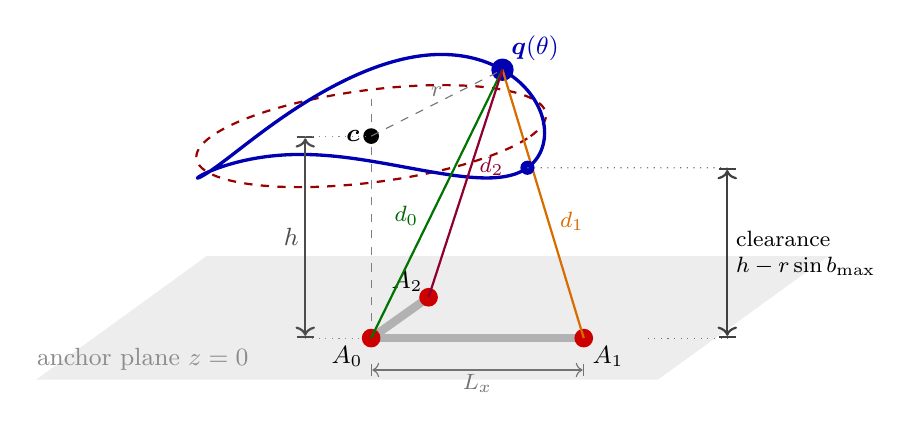
\begin{tikzpicture}[scale=1.35]
  % oblique projection: world (X,Y,Z) -> screen (X + 0.45 Y, 0.32 Y + Z)
  % embedding: b(theta) = 0.35 cos 2theta  ->  20.05 deg = 0.35 rad

  % ground plane
  \fill[black!7] (-3.15,-0.39) -- (2.70,-0.39) -- (4.30,0.77) -- (-1.55,0.77) -- cycle;
  \node[black!45, font=\small] at (-2.15,-0.20) {anchor plane $z=0$};

  % virtual circle (red, dashed) in the plane through c
  \draw[red!60!black, thick, dashed]
     plot[domain=0:360,samples=140]
     ({1.5*cos(\x)+0.675*sin(\x)}, {1.9+0.48*sin(\x)});

  % embedded curve (blue)
  \draw[blue!70!black, very thick]
     plot[domain=0:360,samples=220]
     ({1.5*cos(11.46*cos(2*\x))*cos(\x) + 0.675*cos(11.46*cos(2*\x))*sin(\x)},
      {1.9 + 0.48*cos(11.46*cos(2*\x))*sin(\x) - 1.5*sin(11.46*cos(2*\x))});

  % centre and vertical axis
  \coordinate (C) at (0,1.9);
  \draw[dashed, black!50] (0,0) -- (0,2.25);
  \fill[black] (C) circle (2.1pt);
  \node[font=\small, left, inner sep=4pt] at (C) {$\cv$};

  % h measure
  \draw[|<->|, black!70, thick] (-0.62,0) -- node[left,font=\small,inner sep=2pt] {$h$} (-0.62,1.9);
  \draw[dotted, black!45] (-0.62,0) -- (0,0);
  \draw[dotted, black!45] (-0.62,1.9) -- (0,1.9);

  % template L on the ground
  \draw[line width=3pt, black!30] (0,0) -- (2.0,0);
  \draw[line width=3pt, black!30] (0,0) -- (0.54,0.384);
  \fill[red!80!black] (0,0)          circle (2.5pt);
  \fill[red!80!black] (2.0,0)        circle (2.5pt);
  \fill[red!80!black] (0.54,0.384)   circle (2.5pt);
  \node[font=\small, below left,  inner sep=3pt] at (0,0)        {$A_0$};
  \node[font=\small, below right, inner sep=3pt] at (2.0,0)      {$A_1$};
  \node[font=\small, above left,  inner sep=2pt] at (0.54,0.384) {$A_2$};
  \draw[|<->|, black!55] (0,-0.30) -- node[below,font=\footnotesize,inner sep=1.5pt] {$L_x$} (2.0,-0.30);

  % drone at theta = 65 deg
  \coordinate (D) at (1.235,2.524);
  \fill[blue!70!black] (D) circle (3.0pt);
  \node[blue!70!black, font=\small, above right, inner sep=3pt] at (D) {$\q(\theta)$};

  % radius
  \draw[dashed, black!55] (C) -- node[above,font=\footnotesize,pos=0.5,inner sep=2pt] {$r$} (D);

  % the three ranges, labels pushed apart along their own lines
  \draw[green!45!black,  thick] (0,0)        -- (D);
  \draw[orange!85!black, thick] (2.0,0)      -- (D);
  \draw[purple!75!black, thick] (0.54,0.384) -- (D);
  \node[green!40!black,  font=\footnotesize, left,  inner sep=2pt] at (0.50,1.15)  {$d_0$};
  \node[orange!85!black, font=\footnotesize, right, inner sep=2pt] at (1.72,1.10)  {$d_1$};
  \node[purple!75!black, font=\footnotesize, right, inner sep=1pt] at (0.99,1.62)  {$d_2$};

  % lowest point of the curve (theta = 0) and clearance
  \coordinate (LOW) at (1.470,1.602);
  \fill[blue!70!black] (LOW) circle (1.9pt);
  \draw[dotted, black!55] (LOW) -- (3.35,1.602);
  \draw[dotted, black!55] (2.60,0) -- (3.35,0);
  \draw[|<->|, black!75, thick] (3.35,0) -- (3.35,1.602);
  \node[font=\footnotesize, align=left, right, inner sep=3pt] at (3.35,0.80)
       {clearance\\ $h - r\sin b_{\max}$};

\end{tikzpicture}
\caption{System geometry. The rigid L-template lies in the ground plane $z=0$
with the corner anchor $A_0$ at the origin. The encirclement centre $\cv$ is a
point in the air at altitude $h$; the virtual circle (red, dashed) lies in the
horizontal plane through $\cv$, and the embedded curve (blue) oscillates about
it in elevation according to $b(\theta)$. The lowest point of the curve is
$h - r\sin b_{\max}$ above the anchors. Note that $A_0$ is a physical anchor on
the ground, \emph{not} the encirclement centre: the separation $h$ between them
is what makes the template observable (\S\ref{sec:observability}).}
\label{fig:geometry}
\end{figure}

%==================================================================
\section{Range Structure and Observability}
\label{sec:observability}
%==================================================================

\subsection{The range equations are linear in the centre frame}

Write $\uv = \q - \cv$, so $\norm{\uv}=r$, and let
$\tilde\av_m = \av_m - \cv$ be the anchors expressed in the \emph{centre frame}.
Expanding the range,
\begin{equation}
d_m^2 = \norm{\uv - \tilde\av_m}^2 = r^2 + \norm{\tilde\av_m}^2 - 2\,\tilde\av_m^\top\uv ,
\end{equation}
so that, remarkably, the \emph{on-curve} range equations are exactly linear:
\begin{equation}
\boxed{\;
A\,\uv = \bm\rho,
\qquad
A = \begin{bmatrix}\tilde\av_0^\top \\ \tilde\av_1^\top \\ \tilde\av_2^\top\end{bmatrix},
\qquad
\rho_m = \tfrac{1}{2}\big(r^2 + \norm{\tilde\av_m}^2 - d_m^2\big).
\;}
\label{eq:linear}
\end{equation}
The quadratic term $\norm{\uv}^2$ has been absorbed by the sphere constraint
rather than cancelled by differencing. Everything about observability follows
from the single matrix $A$: the three ranges see the position only through the
three linear functionals $\tilde\av_m^\top\uv$.

\subsection{The observability determinant}

\begin{proposition}[Observability determinant of the L-template]
\label{prop:det}
With the anchors \eqref{eq:anchors} and $\cv = h\ez$,
\begin{equation}
\boxed{\;\Delta \;\triangleq\; \det A \;=\; -\,h\,L_x\,L_y\,\sin\gamma . \;}
\label{eq:det}
\end{equation}
\end{proposition}
\begin{proof}
$\tilde\av_0 = [0,0,-h]^\top$, and
$\tilde\av_1-\tilde\av_0 = [L_x,0,0]^\top$,
$\tilde\av_2-\tilde\av_0 = [L_y\cos\gamma, L_y\sin\gamma,0]^\top$. Row
operations do not change the determinant, so
$\det A = \det[\tilde\av_0;\ \tilde\av_1-\tilde\av_0;\ \tilde\av_2-\tilde\av_0]$.
Expanding along the first row, only the $(1,3)$ entry survives:
$\det A = (-h)\cdot\det\!\begin{bsmallmatrix}L_x & 0\\ L_y\cos\gamma & L_y\sin\gamma\end{bsmallmatrix}
= -h L_x L_y \sin\gamma$.
\end{proof}

Equation~\eqref{eq:det} is the compact statement of the whole design problem.
The template fails to determine the position, in the sense that $A$ becomes
singular, in exactly three ways, and they are visible as the three factors:
\begin{enumerate}
  \item \textbf{Degenerate arms}, $L_x\to0$ or $L_y\to0$ --- an anchor
        coincides with the corner.
  \item \textbf{Collinear anchors}, $\gamma\to0$ or $\pi$ --- the L collapses to
        a line; see \S\ref{sec:whythree}.
  \item \textbf{Coplanar centre}, $h\to0$ --- the encirclement centre descends
        into the anchor plane; see \S\ref{sec:hzero}.
\end{enumerate}
Geometrically, $\det A = 0$ says precisely that the three anchors and the
encirclement centre are coplanar. Because three points are \emph{always}
coplanar, the substantive content is entirely about whether that plane passes
through $\cv$.

\begin{remark}[Two distinct roles for the sphere constraint]
\label{rem:tworoles}
Solving \eqref{eq:linear} as $\uv = A^{-1}\bm\rho$ requires $r$ to be known, so
it is used inside the filter (where $r$ is a state) and for consistency checking,
not for cold initialisation. Its by-product is valuable: since $\norm{\uv}=r$ is
\emph{not} used in the solve, it becomes a free redundancy check,
\begin{equation}
\varepsilon_{\text{sph}} = \big|\;\norm{A^{-1}\bm\rho} - r\;\big| \;\approx\; 0 ,
\label{eq:spherecheck}
\end{equation}
which flags multipath and stale ranges. A general-purpose solver that does not
assume $r$ is given in \S\ref{sec:init}.
\end{remark}

\subsection{The corner anchor is \emph{not} phase-blind when \texorpdfstring{$h>0$}{h>0}}
\label{sec:cornernotblind}

A frequently repeated claim about this geometry is that the corner range
measures radius only and carries no phase information. That is true if and only
if $h=0$.

\begin{proposition}[Phase sensitivity of the corner range]
\label{prop:cornersens}
$\dfrac{\partial d_0}{\partial\theta} = -\dfrac{\tilde\av_0^\top\,\q'(\theta)}{d_0}
 = \dfrac{h\,q_z'(\theta)}{d_0}$, which vanishes identically in $\theta$ if and
only if $h = 0$ (or the curve is planar, $b\equiv\text{const}$).
\end{proposition}
\begin{proof}
Differentiate $d_0^2 = r^2 + \norm{\tilde\av_0}^2 - 2\tilde\av_0^\top\uv$ with
respect to $\theta$, noting $\uv' = \q'$. With
$\tilde\av_0 = [0,0,-h]^\top$ the inner product picks out $-h q_z'$.
\end{proof}

\begin{corollary}[The classical centre-blind result]
If $h=0$, the corner anchor coincides with the encirclement centre,
$d_0 \equiv r$ is constant, and $\partial d_0/\partial\theta \equiv 0$.
\end{corollary}

So the phase-blindness of the corner anchor is not a property of the L-template;
it is a symptom of the degenerate placement $h=0$. In the intended geometry the
corner anchor is a genuine phase sensor. Table~\ref{tab:infoshare} quantifies
it for a representative design.

\begin{table}[htbp]
\centering
\caption{Share of the total Fisher information about $\theta$ contributed by
each range, for $L_x=L_y=0.5$~m, $h=1$~m, $b(\theta)=0.3\cos2\theta$, corner
anchor beneath the centre. The corner anchor supplies roughly a quarter of the
phase information --- not zero.}
\label{tab:infoshare}
\begin{tabular}{lccc}
\toprule
& $d_0$ (corner) & $d_1$ ($x$-arm) & $d_2$ ($y$-arm) \\
\midrule
$r=0.50$~m & $25.4\%$ & $41.9\%$ & $32.7\%$ \\
$r=0.75$~m & $24.2\%$ & $44.1\%$ & $31.7\%$ \\
$r=1.00$~m & $23.3\%$ & $45.3\%$ & $31.4\%$ \\
\bottomrule
\end{tabular}
\end{table}

\subsection{Fisher information and phase observability everywhere on the orbit}

For independent range errors of standard deviation $\sigma$, the Fisher
information about $\theta$ is
\begin{equation}
I(\theta) = \frac{1}{\sigma^2}\sum_{m=0}^{2}
\left(\frac{\partial d_m}{\partial\theta}\right)^{\!2}
= \frac{1}{\sigma^2}\,\big\lVert D^{-1}A\,\q'(\theta)\big\rVert^2 ,
\qquad D = \operatorname{diag}(d_0,d_1,d_2),
\label{eq:fisher}
\end{equation}
which admits the clean lower bound
\begin{equation}
I(\theta) \;\ge\; \frac{\sigma_{\min}^2\!\big(D^{-1}A\big)}{\sigma^2}\,
\norm{\q'(\theta)}^2 .
\label{eq:fisherbound}
\end{equation}
Under Assumption~\ref{as:regular} ($\q'\neq\bm0$) and $\Delta\neq 0$
($A$ invertible), \eqref{eq:fisherbound} is strictly positive for every
$\theta$: \emph{the phase is observable everywhere on the orbit}, with no blind
spots. This is the general replacement for the classical planar argument that
the $x$-arm supplies $\cos\theta$ and the $y$-arm supplies $\sin\theta$, whose
zeros never coincide; that argument is the $h=0$, $b\equiv0$ special case of
\eqref{eq:fisherbound}.

Since $\norm{\q'}\approx r$ for mild embeddings, \eqref{eq:fisherbound} also
gives the scaling that matters in design: $\sigma_\theta \propto 1/r$. A larger
encirclement radius improves phase accuracy.

\subsection{Why three non-collinear anchors}
\label{sec:whythree}

The necessity argument is now a corollary of \eqref{eq:det}, but the mechanism
for the two-anchor case is worth displaying because it defeats a tempting
workaround.

\paragraph{One anchor.} A single range gives one scalar constraint on three
degrees of freedom. With the anchor at the centre it is worse than
under-determined: $d_0\equiv r$ for every $\theta$, so rotating the entire
formation is a continuous gauge freedom and $\theta=0$ is undefined.

\paragraph{Two anchors.} Two spheres intersect in a circle about the
$A_0A_1$ baseline; one rotational degree of freedom survives. In the planar case
both ranges depend on $\theta$ only through the \emph{even} function
$\cos\theta$, so $+\theta$ and $-\theta$ are exactly indistinguishable.

\begin{proposition}[Motion does not resolve the two-anchor ambiguity]
\label{prop:mirror}
Let $\theta(t)$ be any trajectory and $\theta'(t)=-\theta(t)$ its mirror image
about the baseline. Then $d_m(\theta'(t)) = d_m(\theta(t))$ for $m\in\{0,1\}$
and all $t$.
\end{proposition}
\begin{proof}
Both ranges depend on the phase only through $\cos\theta$, and
$\cos(-\theta)=\cos\theta$.
\end{proof}

This is worth stating plainly because it kills an intuitive fix: one might hope
that \emph{knowing} the swarm rotates counter-clockwise disambiguates the
mirror. It does not. A CCW trajectory and its CW mirror generate bit-for-bit
identical range sequences, so the assumed sense cannot be tested against the
data. Breaking an even symmetry requires an odd measurement, which is exactly
what an off-axis third anchor provides (Figure~\ref{fig:ambiguity}).

\paragraph{Three collinear anchors.} No improvement: every anchor on the
baseline shares the same rotational symmetry, and formally $\sin\gamma\to0$ in
\eqref{eq:det}. It is non-collinearity, not anchor count, that breaks the
symmetry.

\begin{figure}[htbp]
\centering
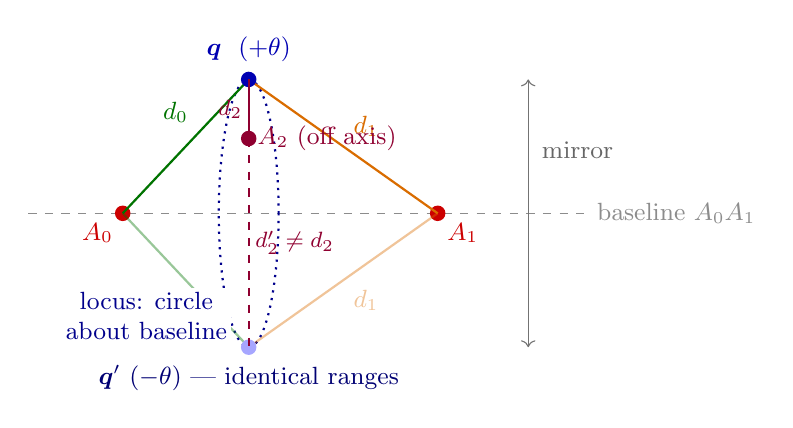
\begin{tikzpicture}[scale=1.0]
  \draw[dashed, black!45] (-1.2,0) -- (5.9,0) node[right, font=\small] {baseline $A_0A_1$};
  \fill[red!80!black] (0,0)   circle (2.8pt) node[below left, font=\small] {$A_0$};
  \fill[red!80!black] (4.0,0) circle (2.8pt) node[below right,font=\small] {$A_1$};

  \draw[blue!55!black, dotted, thick] (1.6,0) ellipse (0.38 and 1.7);
  \coordinate (P)  at (1.6, 1.7);
  \coordinate (Pm) at (1.6,-1.7);

  \draw[green!45!black, thick] (0,0)   -- node[above left, font=\small,pos=0.6] {$d_0$} (P);
  \draw[orange!85!black,thick] (4.0,0) -- node[above right,font=\small,pos=0.5] {$d_1$} (P);
  \draw[green!45!black, thick, opacity=0.4] (0,0)   -- node[below left, font=\small,pos=0.6] {$d_0$} (Pm);
  \draw[orange!85!black,thick, opacity=0.4] (4.0,0) -- node[below right,font=\small,pos=0.5] {$d_1$} (Pm);

  \fill[blue!70!black] (P)  circle (2.8pt);
  \node[blue!70!black, above, font=\small] at ($(P)+(0,0.10)$) {$\q$ \ ($+\theta$)};
  \fill[blue!35!white] (Pm) circle (2.8pt);
  \node[blue!45!black, below, font=\small] at ($(Pm)+(0,-0.10)$) {$\q'$ ($-\theta$) --- identical ranges};

  % third anchor off axis breaks it
  \fill[purple!75!black] (1.6,0.95) circle (2.8pt) node[right, font=\small, inner sep=3pt] {$A_2$ (off axis)};
  \draw[purple!75!black, thick] (1.6,0.95) -- node[left,font=\footnotesize,inner sep=2pt] {$d_2$} (P);
  \draw[purple!75!black, thick, dashed] (1.6,0.95) -- node[right,font=\footnotesize,inner sep=2pt] {$d_2' \ne d_2$} (Pm);

  \node[blue!55!black, font=\small, align=center, fill=white, inner sep=1.5pt]
    at (0.30,-1.30) {locus: circle\\about baseline};
  \draw[<->, black!55] (5.15,1.7) -- (5.15,-1.7);
  \node[black!60, font=\small, right] at (5.2,0.80) {mirror};
\end{tikzpicture}
\caption{The two-anchor mirror ambiguity and its resolution. Every point on the
dotted circle about the $A_0A_1$ baseline produces the same pair $(d_0,d_1)$; in
the encirclement plane this collapses to the exactly indistinguishable pair
$\pm\theta$ (Proposition~\ref{prop:mirror}), which no amount of motion can
separate. An anchor $A_2$ placed \emph{off} the baseline is at different
distances from the two candidates, breaking the symmetry.}
\label{fig:ambiguity}
\end{figure}

%==================================================================
\section{The Degenerate Limit \texorpdfstring{$h\to 0$}{h to 0}}
\label{sec:hzero}
%==================================================================

By \eqref{eq:det}, $\Delta = -hL_xL_y\sin\gamma \to 0$ as the encirclement
centre descends toward the anchor plane. This section works out what actually
breaks --- and, equally important, what does not. The conclusion inverts the
advice usually given.

\subsection{Collapse of the linear solve, and the direction that is lost}

As $h\to0$, $\tilde\av_0 \to \bm0$: the first row of $A$ vanishes and $A$ drops
to rank $2$. Since all three $\tilde\av_m$ then lie in the plane $z=0$, the
kernel is
\begin{equation}
\ker A = \operatorname{span}\{\ez\},
\end{equation}
so the unobservable direction is exactly \emph{vertical}. Writing the solution
of \eqref{eq:linear} in terms of the SVD, the component of $\uv$ along $\ez$ is
reconstructed with gain $\propto 1/h$:
\begin{equation}
\sigma_{u_z} \;\sim\; \frac{\sigma\,d}{h}\,,
\qquad
\sigma_{u_x},\ \sigma_{u_y} \;\sim\; \frac{\sqrt2\,\sigma\,d}{L}\,,
\label{eq:hgain}
\end{equation}
where $d$ is a typical drone-to-anchor range. The horizontal components remain
governed by the template baseline and are unaffected by $h$; only the vertical
estimate diverges.

\subsection{Loss of the sign resolution and of the consistency test}

Two further failures follow from the same geometry.

First, the general (non-sphere) solver of \S\ref{sec:init} determines the
vertical coordinate only up to sign, $\zeta = \pm\sqrt{d_0^2-\alpha^2-\beta^2}$,
resolved by the physical prior that the drone flies above the template. As
$\zeta\to 0$ that prior becomes operationally useless: the discriminant
$d_0^2-\alpha^2-\beta^2$ is a small difference of large numbers, its noise
straddles zero, and a nontrivial fraction of measurement epochs return a
\emph{negative} discriminant which must be rejected outright. The estimator
starves.

Second, the redundancy \eqref{eq:spherecheck} disappears with the rank of $A$.
At $h=0$ the sphere constraint is no longer spare information; it is required to
replace the lost row, and the fault-detection channel is gone.

\subsection{Physical clearance: the binding constraint}

From \eqref{eq:trajectory} the lowest point of the trajectory is
$h - r\sin b_{\max}$, so the curve stays above the anchor plane only if
\begin{equation}
\boxed{\; h \;>\; r\,\sin b_{\max} \;}
\label{eq:clearance}
\end{equation}
and a practical design needs margin beyond this for ground effect, prop wash
over the anchors, and altitude tracking error. For $r=1$~m and
$b_{\max}=0.3$~rad the bare requirement is $h > 0.30$~m.

Violating \eqref{eq:clearance} is not a gentle degradation. The curve crosses
the anchor plane, and since $z(\theta) = h - r\sin b(\theta)$ is periodic, it
crosses \emph{twice per period of $b$} --- four times per revolution for the
representative $b(\theta) = b_{\max}\cos2\theta$. Each crossing is
simultaneously a $\zeta$-sign singularity and a ground strike.

\subsection{What does \emph{not} break: phase observability}

It is natural to assume that because $\Delta\to0$, the phase becomes
unobservable. It does not. Phase depends on the horizontal components, which by
\eqref{eq:hgain} are insensitive to $h$; and reducing $h$ brings the drone
\emph{closer} to the anchors, which by \eqref{eq:fisher} increases
$|\partial d_m/\partial\theta| \propto 1/d_m$. The two effects do not cancel ---
the second wins. Table~\ref{tab:hsweep} gives the numerically evaluated
Cram\'er--Rao bound.

\begin{table}[htbp]
\centering
\caption{Cram\'er--Rao bound on phase, swept over centre altitude.
$L_x=L_y=0.5$~m, $r=1$~m, $b(\theta)=0.3\cos2\theta$, $\sigma=5$~cm; error
scales linearly in $\sigma$. Phase accuracy \emph{improves} monotonically as
$h\to0$, while clearance and the observability determinant collapse. The
binding constraint is clearance, not phase observability.}
\label{tab:hsweep}
\begin{tabular}{lcccc}
\toprule
$h$ [m] & worst-case $\sigma_\theta$ & RMS $\sigma_\theta$ & clearance [m] & $\Delta$ \\
\midrule
$2.00$ & $18.79^\circ$ & $7.31^\circ$ & $+1.70$ & $-0.500$ \\
$1.00$ & $12.63^\circ$ & $6.52^\circ$ & $+0.70$ & $-0.250$ \\
$0.50$ & $11.13^\circ$ & $6.81^\circ$ & $+0.20$ & $-0.125$ \\
$0.25$ & $\ \ 9.99^\circ$ & $6.55^\circ$ & $-0.05$ & $-0.063$ \\
$0.10$ & $\ \ 8.16^\circ$ & $6.32^\circ$ & $-0.20$ & $-0.025$ \\
$0.02$ & $\ \ 8.02^\circ$ & $6.28^\circ$ & $-0.28$ & $-0.005$ \\
\midrule
\multicolumn{5}{l}{\footnotesize Negative clearance = the curve passes through the floor.} \\
\bottomrule
\end{tabular}
\end{table}

\subsection{Design rule for the altitude}

\begin{center}
\fbox{\parbox{0.93\textwidth}{
\textbf{Design rule (altitude).}\;
Choose $h$ as \emph{small} as the following three constraints permit, not as
large as possible:
\emph{(i)} clearance, $h > r\sin b_{\max}$ plus margin;
\emph{(ii)} $\zeta$-sign robustness, which needs the nominal
$\zeta \approx h$ to stand several $\sigma$ clear of zero;
\emph{(iii)} vertical conditioning, $\sigma_{u_z}\sim\sigma d/h$.
Flying higher costs phase accuracy, because it moves the vehicle away from the
anchors. The optimum is broad and flat --- Table~\ref{tab:hsweep} varies by less
than $1^\circ$ RMS across a factor of one hundred in $h$ --- so
$h \approx r$ is a defensible compromise that satisfies all three constraints
with margin, but it should be adopted for constraints \emph{(i)--(iii)} and not
in the mistaken belief that altitude buys phase accuracy.
}}
\end{center}

%==================================================================
\section{Closed-Form Initialisation}
\label{sec:init}
%==================================================================

Cold-starting the filter needs a solution that does not presuppose $r$. Let
$\uv = \q - \av_0 = \q$ in the template frame. Subtracting
$d_0^2 = \norm{\uv}^2$ from the other two range equations cancels the quadratic
term and leaves two linear equations,
\begin{equation}
\bv_1^\top\uv = \tfrac{1}{2}\big(d_0^2 - d_1^2 + \norm{\bv_1}^2\big),
\qquad
\bv_2^\top\uv = \tfrac{1}{2}\big(d_0^2 - d_2^2 + \norm{\bv_2}^2\big),
\end{equation}
which with the anchor coordinates \eqref{eq:anchors} solve as
\begin{equation}
\alpha = \frac{d_0^2 - d_1^2 + L_x^2}{2L_x},
\qquad
\beta = \frac{\tfrac{1}{2}\big(d_0^2-d_2^2+L_y^2\big) - L_y\cos\gamma\;\alpha}{L_y\sin\gamma},
\qquad
\zeta = +\sqrt{\,d_0^2 - \alpha^2 - \beta^2\,},
\label{eq:trilat}
\end{equation}
the positive root being selected by the physical prior of
\S\ref{sec:hzero}. Reject the epoch if the discriminant is negative rather than
clamping it. The phase then follows directly, by Corollary~\ref{cor:exact}, as
\begin{equation}
\theta = \operatorname{atan2}\big(\beta - c_y,\ \alpha - c_x\big)
       = \operatorname{atan2}(\beta,\ \alpha),
\end{equation}
the second equality holding because $\cv = h\ez$ has no horizontal component ---
the corner anchor sits directly beneath the encirclement centre. If the template
is deliberately offset horizontally, subtract $\cv$ first. An initial radius
estimate follows from $\hat r = \norm{[\alpha,\beta,\zeta]^\top - \cv}$.

%==================================================================
\section{Recommended Estimator: EKF in Common and Differential Coordinates}
\label{sec:ekf}
%==================================================================

The algebraic pipeline above is the initialiser, not the tracker. It needs three
simultaneous ranges (two-way ranging delivers them asynchronously) and it
amplifies noise by the GDOP factor of \S\ref{sec:design}. The filter instead
constrains the state to the curve from the outset, reducing three unknowns to
one per agent, and uses only the \emph{forward} embedding evaluation.

\subsection{Coordinates}

Let $\Delta_{\text{nom}} = 2\pi/n$ be the nominal spacing and define the
neighbours' phases as deviations from where the formation says they ought to be,
\begin{equation}
\theta_k = \theta_i + \Delta_{\text{nom}} + \delta_k,
\qquad
\theta_j = \theta_i - \Delta_{\text{nom}} + \delta_j ,
\label{eq:cdcoords}
\end{equation}
so $\delta_k,\delta_j$ are \emph{formation errors}, zero at perfect spacing. The
state is
\begin{equation}
\bm{x} = \big[\,\underbrace{\theta_i}_{\text{common}},\
\underbrace{\delta_k,\ \delta_j}_{\text{differential}},\
\underbrace{\omega_e}_{\text{rate error}},\ r\,\big]^\top ,
\label{eq:cdstate}
\end{equation}
and the quantities the controller consumes follow directly,
\begin{equation}
\varphi^{ki} = -\big(\Delta_{\text{nom}} + \delta_k\big),
\qquad
\varphi^{ji} = +\big(\Delta_{\text{nom}} - \delta_j\big).
\label{eq:cdsep}
\end{equation}

\subsection{Why these coordinates: the process-noise prior}

The transformation adds no information --- it is an exact linear change of
coordinates, $\bm y = T\bm x + \bm c$ with
$T = \begin{bsmallmatrix}1&0&0\\1&1&0\\1&0&1\end{bsmallmatrix}$ --- so a filter
in either set is algebraically identical given $Q_y = TQ_xT^\top$. The gain is
\emph{expressibility}.

In the naive coordinates $[\theta_i,\theta_k,\theta_j]$ a diagonal
$Q=\operatorname{diag}(q,q,q)$ asserts that the separations random-walk
$\sqrt2$ times faster than the individual phases. Physically the opposite holds:
all agents receive the same nominal rate, fly in the same air, and are actively
regulated toward a fixed spacing, so the dominant disturbances --- wind, a
mis-scaled rate command, a systematically slow loop --- displace the formation
\emph{as a whole}. Encoding that belief in the naive coordinates requires
\begin{equation}
Q_y = T\operatorname{diag}(q_c,q_\delta,q_\delta)T^\top =
\begin{bmatrix}
q_c & q_c & q_c \\
q_c & q_c+q_\delta & q_c \\
q_c & q_c & q_c+q_\delta
\end{bmatrix},
\qquad q_\delta \ll q_c ,
\end{equation}
a dense, almost perfectly correlated matrix that nobody reaches by tuning three
diagonal entries. In common/differential coordinates the same belief is ``one
large number and two small ones''.

\subsection{Prediction}

\begin{align}
\theta_{i,t+1} &= \theta_{i,t} + \big(\omega_{z,t}^{i} + \omega_{e,t}\big)\Delta t + w_\theta, \\
\delta_{k,t+1} &= \delta_{k,t} + w_\delta, \qquad \delta_{j,t+1} = \delta_{j,t} + w_\delta, \\
\omega_{e,t+1} &= \omega_{e,t} + w_\omega, \qquad r_{t+1} = r_t + w_r ,
\end{align}
with $Q = \operatorname{diag}(q_\theta,q_\delta,q_\delta,q_\omega,q_r)$,
$q_\delta \ll q_\theta$, and
\begin{equation}
F = \begin{bmatrix}
1&0&0&\Delta t&0\\ 0&1&0&0&0\\ 0&0&1&0&0\\ 0&0&0&1&0\\ 0&0&0&0&1
\end{bmatrix},
\end{equation}
constant and state-independent, so the propagation is exact. Two properties
matter. First, \emph{the neighbours are no longer propagated at an unverifiable
nominal rate}: holding the differences constant carries them along with whatever
the ego agent is actually doing, so common-mode rate error cancels exactly and
never enters the separation prediction. Second, \emph{the rate error is learned,
not assumed}: modelling $\omega_e$ as a random walk absorbs a persistent
commanded-versus-achieved discrepancy that would otherwise appear as a lag bias
in $\theta_i$, which process noise can widen but never shift.

\subsection{Measurement models and Jacobians}

Write $\q_\square = \cv + r\,\hat{\bm u}(\theta_\square)$ with
$\hat{\bm u}(\theta) = \Rot_e(\theta)[\cos\theta,\sin\theta,0]^\top$, so
$\partial\q/\partial r = \hat{\bm u}$. Every range is applied as an independent
\emph{scalar} update as it arrives, matching both the asynchronous nature of
two-way ranging and the existing scalar-update structure of the onboard
estimator.

\paragraph{Anchor ranges.} For $m\in\{0,1,2\}$, with
$\hat{\bm e}_m = (\q_i-\av_m)/\norm{\q_i-\av_m}$,
\begin{equation}
h_m = \norm{\q_i - \av_m},
\quad
\frac{\partial h_m}{\partial\theta_i} = \hat{\bm e}_m^\top \q'(\theta_i),
\quad
\frac{\partial h_m}{\partial r} = \hat{\bm e}_m^\top \hat{\bm u}(\theta_i),
\quad
\frac{\partial h_m}{\partial \delta_k} =
\frac{\partial h_m}{\partial \delta_j} =
\frac{\partial h_m}{\partial \omega_e} = 0 .
\label{eq:janchor}
\end{equation}
By Proposition~\ref{prop:cornersens} the $m=0$ phase Jacobian is $h q_z'/d_0$,
which is \emph{not} zero for $h>0$; no special-casing of the corner anchor is
required or appropriate.

\paragraph{Neighbour chords.} With
$\hat{\bm e}_{ik} = (\q_i-\q_k)/\norm{\q_i-\q_k}$ and $\theta_k$ depending on
$\theta_i$ through \eqref{eq:cdcoords},
\begin{equation}
\frac{\partial h_{ik}}{\partial\theta_i} = \hat{\bm e}_{ik}^\top\big(\q'(\theta_i)-\q'(\theta_k)\big),
\qquad
\frac{\partial h_{ik}}{\partial\delta_k} = -\,\hat{\bm e}_{ik}^\top \q'(\theta_k),
\qquad
\frac{\partial h_{ik}}{\partial r} = \frac{h_{ik}}{r},
\label{eq:jchord}
\end{equation}
symmetrically for $h_{ij}$. The tangent is
\begin{equation}
\q'(\theta) = \frac{d\Rot_e}{d\theta}\pv + \Rot_e\frac{d\pv}{d\theta},
\qquad
\frac{d\Rot_e}{d\theta} = \Rot_e\,\Big[J_r\big(\bm\omega(\theta)\big)\,\frac{d\bm\omega}{d\theta}\Big]_\times ,
\end{equation}
with $J_r$ the right Jacobian of $\SO(3)$; under the design rule of
\S\ref{sec:azimuth} the normal form \eqref{eq:trajectory} can be differentiated
directly instead, and in firmware a central difference of $\q(\theta)$ is an
acceptable substitute for either.

\subsection{The structure this exposes}

\begin{proposition}[Chords are blind to the common mode on the flat circle]
\label{prop:commonblind}
For $\Rot_e\equiv I$, $\partial h_{ik}/\partial\theta_i = 0$ identically.
\end{proposition}
\begin{proof}
Expand
$(\q_i-\q_k)^\top\big(\q'(\theta_i)-\q'(\theta_k)\big)
= \q_i^\top\q'_i + \q_k^\top\q'_k - \q_i^\top\q'_k - \q_k^\top\q'_i$.
The first two vanish by Proposition~\ref{prop:sphere}
($\q^\top\q' = 0$ on a sphere). For the flat circle
$\q_i^\top\q'_k = r^2\sin(\theta_i-\theta_k)$ and
$\q_k^\top\q'_i = r^2\sin(\theta_k-\theta_i) = -\q_i^\top\q'_k$, so the
remaining two cancel. Geometrically: rotating the whole formation rigidly
leaves every chord unchanged.
\end{proof}

\begin{center}
\begin{tabular}{lll}
\toprule
Measurement & Common mode $(\theta_i,\omega_e,r)$ & Differential $(\delta_k,\delta_j)$ \\
\midrule
Anchor ranges $d_0,d_1,d_2$ & \textbf{strong} (all three, incl.\ $d_0$) & none \\
Neighbour chords $d_{ik},d_{ij}$ & weak; zero if $\Rot_e\equiv I$ & \textbf{strong} \\
\bottomrule
\end{tabular}
\end{center}

The two sensor types are \emph{structurally} complementary: the anchors carry
the common mode, which the chords cannot observe on a flat circle and observe
only weakly on a distorted one; the chords carry the differential modes, which
the anchors do not touch at all. The residual common-mode sensitivity of a chord
is precisely the symmetry breaking introduced by the embedding, and should be
treated as a bonus, never as a substitute for the anchors.

\subsection{Assumptions and limitations}

\begin{remark}[The ahead/behind ambiguity]
For the flat circle $d_{ik} = 2r|\sin(\tfrac{\theta_i-\theta_k}{2})|$ is even in
the phase difference, so a chord alone cannot distinguish a neighbour ahead from
one behind. This is resolved at initialisation by the CCW ordering convention
(distinct UWB node IDs for leader and follower) and maintained thereafter by
prediction continuity, a branch switch requiring an innovation large enough to
be gated as an outlier.
\end{remark}

\begin{remark}[A common radius is an assumption, not a measurement]
A single chord cannot separate a neighbour's phase from its radius: a nearer
neighbour at larger separation produces the same chord. The shared-$r$ state
encodes the modelling assumption that all agents hold the commanded radius,
reasonable under active radial control but to be stated explicitly, with $q_r$
tuned to the residual formation-wide radial variation.
\end{remark}

\begin{remark}[Common-mode dominance is an assumption]
Setting $q_\delta \ll q_\theta$ asserts that disturbances are shared. This holds
for wind and rate-scaling errors but not for agent-specific faults (a failing
motor, a diverged local estimator), for which the differential channel is
under-noised and the filter slow to react. Raising $q_\delta$ recovers the
uncorrelated behaviour as the $q_\delta \sim q_\theta$ limit.
\end{remark}

\begin{remark}[What no reformulation repairs]
\label{rem:notfixed}
\emph{(i)} \textbf{Range bias} --- antenna-delay miscalibration or NLOS
propagation yields a confidently wrong estimate; only calibration fixes it.
\emph{(ii)} \textbf{Gross outliers} --- multipath requires an explicit
innovation gate; \eqref{eq:spherecheck} is a cheap additional test.
\emph{(iii)} \textbf{The control law's singularity} --- laws of the form
$\omega = \omega_{z,d} + k(1/\varphi^{ki} + 1/\varphi^{ji})$ diverge as a
separation approaches zero, so with $\sigma_\Delta \approx 10\text{--}30^\circ$
the estimate sits only a few $\sigma$ from a pole that produces large,
sign-flipping rate commands. This is a plausible mechanism for erratic or
apparently stalled motion, and it is a \emph{controller} problem, not an
estimator problem.
\end{remark}

\begin{remark}[Diagnosing which is active]
Log the \textbf{normalized innovation squared} per measurement type against its
$\chi^2$ bound: persistently high indicates an overconfident filter or an
unmodelled bias, persistently low indicates excessive conservatism. Then run the
estimator \textbf{open loop} against ground truth. An estimate that is accurate
open loop but degrades once the loop is closed implicates
Remark~\ref{rem:notfixed}(iii), not the filter.
\end{remark}

%==================================================================
\section{Error Analysis and Template Sizing}
\label{sec:design}
%==================================================================

\subsection{Noise amplification}

Differentiating \eqref{eq:trilat} with respect to the measured ranges and
propagating independent errors of standard deviation $\sigma$ gives
\begin{equation}
\sigma_\alpha \approx \sqrt2\,\frac{d}{L_x}\,\sigma,
\qquad
\sigma_\beta \approx \sqrt2\,\frac{d}{L_y}\,\sigma,
\qquad
\sigma_\theta \approx \frac{\sigma_{xy}}{r},
\label{eq:gdop}
\end{equation}
with $d$ the typical drone-to-anchor distance. Two competing ratios appear, and
both should be checked at design time:
\begin{equation}
\text{baseline ratio } \frac{d}{L} \quad\text{(want small)},
\qquad
\text{phase gain } \frac{1}{r} \quad\text{(want $r$ large)} .
\end{equation}

\begin{center}
\fbox{\parbox{0.93\textwidth}{
\textbf{Design rule (template).}\; Phase error scales as
$\sigma_\theta \sim \sqrt2\,\sigma d/(L r)$. A short baseline \emph{multiplies}
the ranging noise. Aim for $L \gtrsim r$, and prefer equal arms
($L_x=L_y$), which equalises accuracy around the orbit --- unequal arms make the
estimate $L_x/L_y$ times noisier along the long arm's own direction. Distinguish
the arms by anchor \emph{ID}, not by length.
}}
\end{center}

\subsection{Worked numbers}

Table~\ref{tab:sizing} evaluates \eqref{eq:gdop} for $r=1$~m, $h=1$~m
($d\approx1.4$~m) and a representative Crazyflie two-way-ranging noise of
$\sigma = 0.10$~m. The last column gives the exact worst-case Cram\'er--Rao
bound from \eqref{eq:fisher}, which is slightly better than the GDOP estimate
because it credits the phase information carried by the corner anchor
(Table~\ref{tab:infoshare}) that \eqref{eq:gdop} discards.

\begin{table}[htbp]
\centering
\caption{Template sizing at $r=1$~m, $h=1$~m, $\sigma=0.10$~m. Errors scale
linearly in $\sigma$: halving the ranging noise halves every entry.}
\label{tab:sizing}
\begin{tabular}{lccccl}
\toprule
Template & $L_x$ & $L_y$ & $\sigma_\alpha$ & $\sigma_\theta$ (GDOP) & CRLB, worst case \\
\midrule
3D-printed, small  & $0.30$~m & $0.30$~m & $0.66$~m & $\approx 38^\circ$ & --- \\
As currently planned & $0.50$~m & $0.50$~m & $0.40$~m & $\approx 23^\circ$ & $19.7^\circ$ \\
Rod / tripod rig   & $1.00$~m & $1.00$~m & $0.20$~m & $\approx 11^\circ$ & --- \\
Room-scale         & $2.00$~m & $2.00$~m & $0.10$~m & $\approx \ 6^\circ$ & --- \\
\bottomrule
\end{tabular}
\end{table}

The currently planned $0.5$~m arms give $L/r = 0.5$, below the recommended
$L\gtrsim r$, and a worst-case phase error near $20^\circ$ at $\sigma=10$~cm.
Since the nominal inter-agent separation for $n=3$ is $120^\circ$, this is
survivable for the controller but leaves little margin against
Remark~\ref{rem:notfixed}(iii). Three levers are available, in decreasing order
of effectiveness: lengthen the arms ($\sigma_\theta \propto 1/L$), reduce the
ranging noise by antenna-delay calibration ($\propto\sigma$), and enlarge the
encirclement radius ($\propto 1/r$). Reducing $r$ makes it worse.

%==================================================================
\section{Implementation Summary}
%==================================================================

\begin{enumerate}
  \item \textbf{Design the embedding tangentially.} Set
        $\bm\omega(\theta) = b(\theta)\that(\theta)$ with $b$ $2\pi$-periodic
        and $|b| < \pi/2$. This makes $\theta=\operatorname{atan2}$ exact
        (Corollary~\ref{cor:exact}), removes all iteration, and wastes no
        control authority (Proposition~\ref{prop:radialnoop}).
  \item \textbf{Calibrate the template offline.} Broadcast-only anchors cannot
        self-calibrate; measure $L_x, L_y, \gamma$ from CAD or physically to a
        few millimetres. Rigidity matters, squareness does not
        (Remark~\ref{rem:selfcal}).
  \item \textbf{Size the template.} $L \gtrsim r$, equal arms, verify against
        Table~\ref{tab:sizing} before building.
  \item \textbf{Choose the altitude.} $h > r\sin b_{\max}$ plus margin
        \eqref{eq:clearance}, and $\zeta \approx h$ several $\sigma$ clear of
        zero. Do not fly higher than these require: altitude costs phase
        accuracy (Table~\ref{tab:hsweep}).
  \item \textbf{Assign node IDs.} Unique IDs for the three anchors and every
        agent; leader/follower roles fixed by the CCW ordering convention.
  \item \textbf{Initialise} with \eqref{eq:trilat} then
        $\theta=\operatorname{atan2}(\beta,\alpha)$, seeding $\theta_k,\theta_j$
        from the chords on the convention-selected branch.
  \item \textbf{Track} with the EKF of \S\ref{sec:ekf}, state
        $[\theta_i,\delta_k,\delta_j,\omega_e,r]$, each range an asynchronous
        scalar update with Jacobians \eqref{eq:janchor}--\eqref{eq:jchord}.
        Tune $q_\delta \ll q_\theta$. Do \emph{not} special-case the corner
        anchor as radius-only.
  \item \textbf{Gate and cross-check.} Reject negative discriminants in
        \eqref{eq:trilat} rather than clamping; apply the sphere-consistency
        test \eqref{eq:spherecheck}; gate innovations.
  \item \textbf{Validate before trusting.} Log NIS per measurement type and run
        the estimator open loop against ground truth before closing the control
        loop. Calibrate antenna delay first --- no filter formulation repairs
        bias.
\end{enumerate}

\end{document}